%\documentclass[standard,
%               backaddress=off,
%               foldmarks=false,
%               enlargefirstpage,
%               pagenumber=off,
%               parskip=half
%               ]{scrlttr2}
%
%\setkomavar{fromname}{Gabriel Hassler}
%\setkomavar{fromaddress}{Department of Computational Medicine / UCLA \\ 5303 Life Sciences \\ Box 951766 \\ Los Angeles, CA 90095}
%\setkomavar{fromphone}{(202) 557-5140}
%\setkomavar{fromemail}{ghassler@g.ucla.edu}
%%\setkomavar{department}{Department of Computational Medicine}


\documentclass[12pt]{article}

\usepackage{amssymb}
\usepackage{geometry}
\usepackage{url}
\geometry{letterpaper} % or letterpaper (US) or a5paper or....
\geometry{margin=1in} % for example, change the margins to 2 inches all round
\usepackage[table]{xcolor}

\newenvironment{reply}{$\triangleright$\bfseries}{$\triangleleft$}
\renewenvironment{quote}
               {\list{}{\rightmargin\leftmargin}%
                \item\relax\normalfont}
               {\endlist}

%
%\newcommand{\bibsection}[1]{}
%\newcommand{\section}[1]{}
%\newcommand{\newblock}{}
%
%   \newenvironment{thebibliography}[1]%
%      {References\begin{description}}{\end{description}}
%   \newcommand{\htmlbibitem}[2]{\label{#2}\item[{[#1]}]}
\usepackage{natbib}
\usepackage[colorlinks, citecolor={blue}]{hyperref}
\usepackage{amsmath}
\usepackage{float}
\usepackage{bm}
\usepackage{graphicx}
\usepackage{subcaption}
\usepackage{setspace}
\usepackage{xr}
\usepackage[textsize=tiny]{todonotes}
\usepackage{algorithm,algorithmicx,algpseudocode}
%\usepackage{subfigure}
\setlength{\parindent}{0pt}
\setlength{\parskip}{12pt}

\usepackage{braket}


\usepackage{amsthm}

\definecolor{trevorblue}{rgb}{0.330, 0.484, 0.828}
\definecolor{trevoryellow}{rgb}{0.829, 0.680, 0.306}


\def\suppDoc{main}
\externaldocument{\suppDoc}
%\input{missing_traits_supplement_revision.xtr}
%\input{revision_values.sty}
%\input{new_floats.tex}

\usepackage{makecell}
\usepackage{booktabs}
\usepackage{multirow}
\usepackage{bm}

\usepackage{todonotes}

\newcommand{\mb}{\mathbf}
\newcommand{\mc}{\mathcal}
\newcommand{\dx}{\mbox{d}}

\newcommand{\argmax}{\operatornamewithlimits{argmax}}
\newcommand*{\fplus}{\genfrac{}{}{0pt}{}{}{+}}
\newcommand*{\fdots}{\genfrac{}{}{0pt}{}{}{\cdots}}


\renewcommand{\vec}[1]{\mathbf{#1}}
\newcommand{\numTaxa}{N}
\newcommand{\numTraits}{D}
\newcommand{\numDatasets}{M}
%\newcommand{\numLatent}{D}
\newcommand{\taxonIndex}{i}
\newcommand{\traitIndex}{j}
\newcommand{\traitData}{\vec{Y}}
\newcommand{\traitDatum}{y}
\newcommand{\datasetIndex}{m}
\newcommand{\exemplar}{\text{e}}

\newcommand{\sequences}{\vec{S}}
\newcommand{\latentData}{\vec{X}}
\newcommand{\latentdata}{\vec{z}}
\newcommand{\latentDatum}{x}
\newcommand{\phylogeneticParameters}{\boldsymbol{\phi}}
\newcommand{\phylogeny}{{\cal G}}
\newcommand{\tree}{\phylogeny}
%\newcommand{\otherParameters}{\boldsymbol{\
\newcommand{\transpose}{^{t}}

\newcommand{\distanceMatrix}{\mathbf{Y}}
\newcommand{\distance}{y}
\newcommand{\summant}{r}



\newcommand{\cdensity}[2]{\ensuremath{p(#1 \,|\,#2)}}
\newcommand{\density}[1]{\ensuremath{p(#1 )}}

\newcommand{\treeNode}{\nu}

\newcommand{\traitVariance}{\mathbf{\Sigma}}
\newcommand{\nodeIndex}{c}
%\newcommand{\parent}[1]{\mbox{\tiny pa}(#1)}
\newcommand{\parentBig}[1]{\mbox{pa}(#1)}

\newcommand{\sibling}[1]{\mbox{\tiny sib}(#1)}
\newcommand{\siblingBig}[1]{\mbox{sib}(#1)}

\newcommand{\rootMean}{\boldsymbol{\mu}_0}
\newcommand{\rootVarianceScalar}{\tau_0}
\newcommand{\unsequencedVarianceScalar}{\tau_{\exemplar}}
\newcommand{\treeVariance}{\vec{V}_{\tree}}
\newcommand{\hatTreeVariance}{\hat{\vec{V}}_{\tree}}
\newcommand{\mdsSD}{\sigma}
\newcommand{\mdsVariance}{\mdsSD^2}
\newcommand{\residual}{\hat{\traitDatum}}
\newcommand{\modelDistance}{\delta}
\newcommand{\cdf}{\phi}
\newcommand{\normalCDF}[1]{\Phi \left( #1 \right)}

\newcommand{\order}[1]{{\cal O}\hspace{-0.2em}\left( #1 \right)}

\newcommand{\rootNode}{\nu^{\datasetIndex}_{2 \numTaxa_{\datasetIndex} -1 }}
\newcommand{\pathLength}[1]{d(F, #1 )}
\newcommand{\pathLengthNew}[2]{
	d_{F}
	(
	{#1}, {#2}
	)
}
\newcommand{\J}{\vec{J}}
\newcommand{\pprime}{^{\prime}}
\newcommand{\otherIndex}{i \pprime}
\def\kronecker{\raisebox{1pt}{\ensuremath{\:\otimes\:}}}

\newcommand{\x}{\mathbf{x}}

%\graphicspath{{../../Graphs/}}

\def\journalName{Journal of Multivariate Analysis}
\def\journalAbbr{JMVA}
\def\editor{Hongyu Zhao}
\def\editorTitle{Theory and Methods Co-Editor}
\def\editorLast{Zhao}
\def\pubOrg{American Statistical Association}
\def\pubAddressOne{732 North Washington Street}
\def\pubAddressTwo{Alexandria, VA 22314-1943}

\def\paperTitle{A quantum parallel Markov chain Monte Carlo}
\def\paperID{JCGS-22-275}

%\newcommand{\bigo}[1]{\cal{O}\hspace{-.5mm}\left(#1\right)}
\onehalfspacing

\renewcommand{\x}{\mathbf{x}}
\renewcommand{\v}{\mathbf{v}}
\newcommand{\TTheta}{\boldsymbol{\theta}}
\newcommand{\TTTheta}{\boldsymbol{\Theta}}
\newcommand{\tr}{\mbox{tr}}
\newcommand{\X}{\mathbf{X}}

\usepackage{tikz}
\usetikzlibrary{matrix}
\usetikzlibrary{backgrounds}
\usetikzlibrary{calc}
\usetikzlibrary{arrows,shapes}
\usetikzlibrary{decorations}
\usetikzlibrary{decorations.pathmorphing}
\usetikzlibrary{fit}
\usetikzlibrary{decorations.pathreplacing}
\usetikzlibrary{shapes.misc}
\usetikzlibrary{shapes.geometric}

\newtheorem{thm}{Theorem}
\newtheorem{lemma}{Lemma}
\newtheorem{prop}{Proposition}
\newtheorem{cor}{Corollary}
\newtheorem{remark}{Remark}
\newtheorem{example}{Example}
\newtheorem{mydef}{Definition}
\newtheorem*{assumption}{Assumption}
\newtheorem{clm}{Claim}


\begin{document}

%% !TeX document-id = {d42653b9-9ea4-48c2-860b-3d6e6e9d8ab0}
% !TeX TXS-program:compile = txs:///pdflatex/[--shell-escape]
\documentclass[12pt]{article} % For LaTeX2e
%\usepackage{neurips_2021}
\usepackage[colorlinks, citecolor={blue}]{hyperref}
\usepackage{url}
\usepackage{amsfonts,amscd,amssymb}
\usepackage{amsthm,amsmath,natbib}
\usepackage{mathtools}
\DeclarePairedDelimiter{\ceil}{\lceil}{\rceil}
\usepackage{algorithm2e}
\usepackage{bm}
\usepackage{bbm} %bb font numbers
\usepackage[table]{xcolor}
\usepackage{verbatim}
\usepackage{graphicx}
\usepackage{setspace}
\usepackage{natbib}
\usepackage[margin=1in]{geometry}
\usepackage{enumitem}
%\usepackage[nolists]{endfloat}
\usepackage{listings}
\usepackage[textsize=tiny]{todonotes}
\usepackage{tikz}
\usetikzlibrary{shapes.misc}
\usepackage{etoolbox}
\usepackage{appendix}
\usepackage[format=plain,
labelfont={it},
textfont=it]{caption}
\usepackage{subcaption}
\usepackage{wrapfig}
\usepackage{xr}
\usepackage{booktabs}
\usepackage{multirow}
\usepackage{authblk}
\usepackage{mathbbol}
\usepackage{braket}
\usepackage[cache=false]{minted}



\usetikzlibrary{matrix}
\usetikzlibrary{backgrounds}
\usetikzlibrary{calc}
\usetikzlibrary{arrows,shapes}
\usetikzlibrary{decorations}
\usetikzlibrary{decorations.pathmorphing}
\usetikzlibrary{fit}
\usetikzlibrary{decorations.pathreplacing}

\newtoggle{quickdraw}
\toggletrue{quickdraw} % Uncomment this to render more quickly (non-random)


\definecolor{lightgrey}{rgb}{0.9,0.9,0.9}
\definecolor{darkgreen}{rgb}{0,0.3,0}
%\definecolor{darkred}{rgb}{0.3,0,0}

\definecolorset{rgb}{}{}{darkred,0.8,0,0;darkgreen,0,0.5,0;darkblue,0,0,0.5}

%\doublespacing

\SetKwComment{Comment}{/* }{ */}
%\RestyleAlgo{ruled}

\newtheorem{thm}{Theorem}
\newtheorem{lemma}{Lemma}
\newtheorem{prop}{Proposition}
\newtheorem{cor}{Corollary}
\newtheorem{remark}{Remark}
\newtheorem{example}{Example}
\newtheorem{mydef}{Definition}
\newtheorem*{assumption}{Assumption}
\newtheorem{clm}{Claim}

\newcommand{\argmax}{\operatornamewithlimits{arg\,max}}
\newcommand{\argmin}{\operatornamewithlimits{arg\,min}}
\newcommand*{\fplus}{\genfrac{}{}{0pt}{}{}{+}}
\newcommand*{\fdots}{\genfrac{}{}{0pt}{}{}{\cdots}}
\newcommand{\mb}{\mathbf}
\newcommand{\mc}{\mathcal}
\newcommand{\dx}{\mbox{d}}

\renewcommand{\vec}[1]{\mathbf{#1}}
\newcommand{\numTaxa}{N}
\newcommand{\numTraits}{D}
\newcommand{\numDatasets}{M}
%\newcommand{\numLatent}{D}
\newcommand{\taxonIndex}{i}
\newcommand{\traitIndex}{j}
\newcommand{\traitData}{\vec{Y}}
\newcommand{\traitDatum}{y}
\newcommand{\datasetIndex}{m}
\newcommand{\exemplar}{\text{e}}

\newcommand{\sequences}{\vec{S}}
\newcommand{\latentData}{\vec{X}}
\newcommand{\latentdata}{\vec{x}}
\newcommand{\latentDatum}{x}
\newcommand{\phylogeneticParameters}{\boldsymbol{\phi}}
\newcommand{\phylogeny}{{\cal G}}
\newcommand{\tree}{\phylogeny}
%\newcommand{\otherParameters}{\boldsymbol{\
\newcommand{\transpose}{^{t}}

\newcommand{\distanceMatrix}{\mathbf{Y}}
\newcommand{\distance}{y}
\newcommand{\summant}{r}



\newcommand{\cdensity}[2]{\ensuremath{p(#1 \,|\,#2)}}
\newcommand{\density}[1]{\ensuremath{p(#1 )}}

\newcommand{\treeNode}{\nu}

\newcommand{\traitVariance}{\mathbf{\Sigma}}
\newcommand{\nodeIndex}{c}

%\newcommand{\parent}[1]{\mbox{\tiny pa}(#1)}
\newcommand{\parentBig}[1]{\mbox{pa}(#1)}

\newcommand{\sibling}[1]{\mbox{\tiny sib}(#1)}
\newcommand{\siblingBig}[1]{\mbox{sib}(#1)}

\newcommand{\rootMean}{\boldsymbol{\mu}_0}
\newcommand{\rootVarianceScalar}{\tau_0}
\newcommand{\unsequencedVarianceScalar}{\tau_{\exemplar}}
\newcommand{\treeVariance}{\vec{V}_{\tree}}
\newcommand{\hatTreeVariance}{\hat{\vec{V}}_{\tree}}
\newcommand{\mdsSD}{\sigma}
\newcommand{\mdsVariance}{\mdsSD^2}
\newcommand{\residual}{\hat{\traitDatum}}
\newcommand{\modelDistance}{\delta}
\newcommand{\cdf}{\phi}
\newcommand{\normalCDF}[1]{\Phi \left( #1 \right)}

\newcommand{\order}[1]{{\cal O}\hspace{-0.2em}\left( #1 \right)}

\newcommand{\rootNode}{\nu^{\datasetIndex}_{2 \numTaxa_{\datasetIndex} -1 }}
\newcommand{\pathLength}[1]{d(F, #1 )}
\newcommand{\pathLengthNew}[2]{
d_{F}
(
{#1}, {#2}
)
}
\newcommand{\J}{\vec{J}}
\newcommand{\pprime}{^{\prime}}
\newcommand{\otherIndex}{i \pprime}
\def\kronecker{\raisebox{1pt}{\ensuremath{\:\otimes\:}}}

\definecolor{trevorblue}{rgb}{0.330, 0.484, 0.828}
\definecolor{trevoryellow}{rgb}{0.829, 0.680, 0.306}

%%%
%% LaTeX source to reference manuscript changes in revision letters
%%
%% In the manuscript file:
%% 1. Include this file 
%%      %%
%% LaTeX source to reference manuscript changes in revision letters
%%
%% In the manuscript file:
%% 1. Include this file 
%%      \input{make-edits}
%% 2. Define manuscript modifications as
%%      \myedit{UniqueLabel}{Text to appear in manuscript and revision letter}
%%
%% In the revision letter file:
%% 1. Include the automatically updated modifications file
%%      \input{jobname.xtr}
%% 2. Include modified text with
%%      \myeditUniqueLabel
%%
%% Marc A. Suchard
%% 24-Jul-2006
%%

\newwrite\XTR
\AtBeginDocument{\immediate\openout\XTR\jobname.xtr}
\AtEndDocument{\immediate\closeout\XTR}

\newcommand{\myedit}[2]{ % first options is a label, second options is the text
\parbox{0em}{
\shipout\box1{
  \def\mynamea{myedit#1}
  \def\mynameb{\csname \mynamea\endcsname}
\write\XTR{
      \string\newcommand
{\csname myedit#1\endcsname}
}
\write\XTR{
         {``\expandafter\string#2''
         (pg.\string~\thepage)}
}
%\write\XTR{
%    (pg.\string~\thepage)
%}
}
%\hspace*{-1in}
}
%
%\def\thistext{\noexpand#2}
%  \immediate\write\XTR{
%   %     \begin{verbatim}
%        \thistext
%   %     \end{verbatim}
%  }
%\endgroup
%}
%\shipout\vbox{0}
%        \label{\expand\mylabel}
%        \thepage
%  \mylabel
%  \hspace*{-0em}
%  {\bf#2}
#2
}

\newcommand{\myeditblank}[2]{ % first options is a label, second options is the text
\parbox{1em}{
\shipout\box1{
  \def\mynamea{myedit#1}
  \def\mynameb{\csname \mynamea\endcsname}
\write\XTR{
      \string\newcommand
{\csname myedit#1\endcsname}
}
\write\XTR{
         {\expandafter\string#2
         (pg.\string~\thepage)}
}
%\write\XTR{
%    (pg.\string~\thepage)
%}
}
%\hspace*{-1in}
}
%
%\def\thistext{\noexpand#2}
%  \immediate\write\XTR{
%   %     \begin{verbatim}
%        \thistext
%   %     \end{verbatim}
%  }
%\endgroup
%}
%\shipout\vbox{0}
%        \label{\expand\mylabel}
%        \thepage
%  \mylabel
%  \hspace*{-1em}
%  {\bf#2}
}



%\newlength{\strikewidth}
%\newlength{\strikelength}
%\setlength{\strikewidth}{1pt}

%\newcommand{\remove}[1]{
%    \settowidth{\strikelength}{#1}
%    #1\hspace{-\strikelength}
%    \rule[0.5ex]{\strikelength}{\strikewidth}
%}

%\usepackage{ulem}
%\newcommand{\remove}[1]{\sout{#1}}
\newcommand{\remove}[1]{\hspace*{-1em}}

\newcommand{\add}[1]{
%        {\bf #1}
#1%\hspace*{0em}
}


%% 2. Define manuscript modifications as
%%      \myedit{UniqueLabel}{Text to appear in manuscript and revision letter}
%%
%% In the revision letter file:
%% 1. Include the automatically updated modifications file
%%      \input{jobname.xtr}
%% 2. Include modified text with
%%      \myeditUniqueLabel
%%
%% Marc A. Suchard
%% 24-Jul-2006
%%

\newwrite\XTR
\AtBeginDocument{\immediate\openout\XTR\jobname.xtr}
\AtEndDocument{\immediate\closeout\XTR}

\newcommand{\myedit}[2]{ % first options is a label, second options is the text
\parbox{0em}{
\shipout\box1{
  \def\mynamea{myedit#1}
  \def\mynameb{\csname \mynamea\endcsname}
\write\XTR{
      \string\newcommand
{\csname myedit#1\endcsname}
}
\write\XTR{
         {``\expandafter\string#2''
         (pg.\string~\thepage)}
}
%\write\XTR{
%    (pg.\string~\thepage)
%}
}
%\hspace*{-1in}
}
%
%\def\thistext{\noexpand#2}
%  \immediate\write\XTR{
%   %     \begin{verbatim}
%        \thistext
%   %     \end{verbatim}
%  }
%\endgroup
%}
%\shipout\vbox{0}
%        \label{\expand\mylabel}
%        \thepage
%  \mylabel
%  \hspace*{-0em}
%  {\bf#2}
#2
}

\newcommand{\myeditblank}[2]{ % first options is a label, second options is the text
\parbox{1em}{
\shipout\box1{
  \def\mynamea{myedit#1}
  \def\mynameb{\csname \mynamea\endcsname}
\write\XTR{
      \string\newcommand
{\csname myedit#1\endcsname}
}
\write\XTR{
         {\expandafter\string#2
         (pg.\string~\thepage)}
}
%\write\XTR{
%    (pg.\string~\thepage)
%}
}
%\hspace*{-1in}
}
%
%\def\thistext{\noexpand#2}
%  \immediate\write\XTR{
%   %     \begin{verbatim}
%        \thistext
%   %     \end{verbatim}
%  }
%\endgroup
%}
%\shipout\vbox{0}
%        \label{\expand\mylabel}
%        \thepage
%  \mylabel
%  \hspace*{-1em}
%  {\bf#2}
}



%\newlength{\strikewidth}
%\newlength{\strikelength}
%\setlength{\strikewidth}{1pt}

%\newcommand{\remove}[1]{
%    \settowidth{\strikelength}{#1}
%    #1\hspace{-\strikelength}
%    \rule[0.5ex]{\strikelength}{\strikewidth}
%}

%\usepackage{ulem}
%\newcommand{\remove}[1]{\sout{#1}}
\newcommand{\remove}[1]{\hspace*{-1em}}

\newcommand{\add}[1]{
%        {\bf #1}
#1%\hspace*{0em}
}


%\makeatletter
%\def\title@font{\Huge}
%\let\ltx@maketitle\@maketitle
%\def\@maketitle{\bgroup%
%	\let\ltx@title\@title%
%	\def\@title{\resizebox{\textwidth}{!}{%
%			\mbox{\title@font\ltx@title}%
%	}}%
%	\ltx@maketitle%
%	\egroup}
%\makeatother


\title{A quantum parallel Markov chain Monte Carlo}
\date{}



\author{Andrew J.~Holbrook}


\affil{UCLA Biostatistics}





\renewcommand\Authands{ and }


\graphicspath{{figures/}}

\begin{document}


\maketitle




\begin{abstract}

We propose a novel quantum computing strategy for \emph{parallel MCMC} algorithms that generate multiple proposals at each step. This strategy makes parallel MCMC amenable to quantum parallelization by using the Gumbel-max trick to turn the generalized accept-reject step into a discrete optimization problem.  This allows us to embed target density evaluations within a well-known extension of Grover's quantum search algorithm.  Letting $P$ denote the number of proposals in a single MCMC iteration, the combined strategy reduces the number of target evaluations required from $\order{P}$ to $\order{P^{1/2}}$.  In the following, we review both the rudiments of quantum computing and the Gumbel-max trick in order to elucidate their combination for as wide a readership as possible. 


\end{abstract}


\section{Introduction}

\newcommand{\ttheta}{\boldsymbol{\theta}}
\newcommand{\dd}{\mbox{d}}
\newcommand{\ppsi}{\boldsymbol{\psi}}
\newcommand{\U}{\mathbf{U}}
\newcommand{\I}{\mathbf{I}}
\renewcommand{\H}{\mathbf{H}}
\newcommand{\A}{\mathbf{A}}
\newcommand{\B}{\mathbf{B}}
\newcommand{\G}{\mathbf{G}}
\newcommand{\ppi}{\boldsymbol{\pi}}
\newcommand{\llambda}{\boldsymbol{\lambda}}

Parallel MCMC techniques use multiple proposals to obtain efficiency gains over MCMC algorithms such as Metropolis-Hastings \citep{metropolis1953equation,hastings1970monte} and its progeny that use only a single proposal.  \citet{neal2003markov} first develops efficient MCMC transitions for inferring the states of hidden Markov models by proposing a `pool' of candidate states and using dynamic programming to select among them. Next, \citet{tjelmeland2004using} considers inference in the general setting and shows how to maintain detailed balance for an arbitrary number $P$ of proposals.  Consider a probability distribution $\pi(\dd\ttheta)$ defined on $\mathbb{R}^D$ that admits a probability density $\pi(\ttheta)$ with respect to the Lebesgue measure, i.e., $\pi(\dd \ttheta)=:\pi(\ttheta)\dd\ttheta$. To generate samples from the target distribution $\pi$, we craft a kernel $P(\ttheta_0,\dd \ttheta)$ that satisfies
\begin{align}\label{eq:fixes}
\pi(A) = \int \pi(\dd \ttheta_0) P(\ttheta_0,A) \, \quad a.s.
\end{align} 
for  $A \subset \mathbb{R}^D$ for which $\pi(A) > 0$.  Letting $\ttheta_0$ denote the current state of the Markov chain, \citet{tjelmeland2004using} proposes sampling from such a kernel $P(\ttheta_0,\cdot)$ by drawing $P$ proposals $\ttheta_1,\dots,\ttheta_P$ from a distribution $Q(\ttheta_0,\dd \ttheta) =: q(\ttheta_0,\ttheta)\dd \ttheta$ and selecting the next Markov chain state from among the current and proposed states with probabilities
\begin{align}\label{eq:probs}
\pi_p = \frac{\pi(\ttheta_p) \prod_{p' \neq p} q(\ttheta_p,\ttheta_{p'})}{\sum_{p''=0}^P \pi(\ttheta_{p''}) \prod_{p' \neq p''} q(\ttheta_{p''},\ttheta_{p'})} \, , \quad p=0,\dots,P \, .
\end{align}
\citet{tjelmeland2004using} shows that the kernel $P(\ttheta_0,\cdot)$ constructed in such a manner maintains detailed balance and hence satisfies Equation \eqref{eq:fixes}.  Others have since built on this work, developing parallel MCMC methods that generate or recycle multiple proposals \citep{frenkel2004speed,delmas2009does,calderhead2014general,yang2018parallelizable,luo2019multiple,schwedes2021rao,holbrook2021generating}.  
These developments demonstrate the ability of parallel MCMC methods to alleviate inferential challenges such as multimodality and to deliver performance gains over single-proposal competitors as measured by reduced autocorrelation between samples.  In the following, we focus on the specification presented in Algorithm \ref{alg:pMCMC} but note that the techniques we present may also be effective for generalizations of this basic algorithm.

\begin{algorithm}[t!]
	\caption{Parallel MCMC \citep{tjelmeland2004using}}\label{alg:pMCMC}
	\KwData{Initial Markov chain state $\ttheta^{(0)}$; total length of Markov chain $S$; total number of proposals per iteration $P$; routine for evaluating target density $\pi(\cdot)$; routines for drawing random samples from the proposal distribution $Q(\ttheta^{(s)},\cdot)$ and from a $P+1$ discrete distribution $Discrete(\ppi)$ given some probability vector $\ppi=(\pi_0,\dots,\pi_P)$.}
	\KwResult{A Markov chain $\ttheta^{(1)}, \dots, \ttheta^{(S)}$.}
	\For{$s \in\{1,\dots,S\}$}{
		%$\sigma_\pi \gets 0$\;
		$\ttheta_0 \gets \ttheta^{(s-1)}$\;
		\For{$p' \in \{1,\dots,P\}$}{
			$\ttheta_{p'} \gets Q(\ttheta^{(s-1)},\cdot)$\;
		}
		\For{$p' \in \{0,\dots,P\}$}{
			$\pi_{p'} \gets \pi(\ttheta_{p'}) \prod_{p''\neq p'}q(\ttheta_{p'},\ttheta_{p''})$\; 
		}
		$p \gets Discrete(\ppi/\ppi^T\mathbb{1})$\;
		$\ttheta^{(s)} \gets \ttheta_p$\;
	}
	\Return{$\ttheta^{(1)}, \dots, \ttheta^{(S)}$}\ .
	\vspace{0.5em}
	
\end{algorithm}

But the real promise and power of parallel MCMC comes from its natural parallelizability \citep{calderhead2014general}.  Contemporary hardware design emphasizes architectures that enable execution of multiple mathematical operations simultaneously. Parallel MCMC techniques stand to leverage technological developments that keep modern computation on track with Moore's Law, which predicts that processing power doubles every two years.  For example, the algorithm of \citet{tjelmeland2004using} generates $P$ conditionally independent proposals and then evaluates the probabilities of Equation \eqref{eq:probs}.  One may parallelize the proposal generation step using parallel pseudorandom number generators (PRNG) such as those advanced in \citet{salmon2011parallel}. The computational complexity of the target evaluations $\pi(\ttheta_p)$ is linear in the number of proposals. This presents a significant burden when $\pi(\cdot)$ is computationally expensive, e.g., in big data settings or for Bayesian inversion, but evaluation of the target density over the $P$ proposals is again a naturally parallelizable task.  Moreover, widely available machine learning software such as \textsc{TensorFlow} allows users to easily parallelize both random number generation and target evaluations on general purpose graphics processing units (GPU) \citep{lao2020tfp}. Finally, the pairwise evaluations of the proposal density $q(\cdot,\cdot)$ in Equation \eqref{eq:probs} are $\order{P^2}$, but \citet{massive} demonstrate the natural parallelizability of such pairwise operations, obtaining orders-of-magnitude speedups with contemporary GPUs.




While parallel MCMC algorithms are increasingly well-suited for developing many-core computational architectures, there are trade-offs that need to be taken into account when choosing how to allocate computational resources.  On one end of the spectrum, \citet{gelman1992inference} demonstrate the usefulness of generating, combining and comparing multiple independent Markov chains that target the same distribution, and one may perform this embarrassingly parallel task by assigning the operations for each individual chain to a separate central processing unit (CPU) core or GPU work-group.  In this multi-chain context, simultaneously running multiple parallel MCMC chains could limit resources available for the within-chain parallelization described in the previous paragraph.  On the other end of the spectrum, one may find it useful to allocate resources to overcome computational bottlenecks within a single Markov chain that uses a traditional accept-reject step. In big data contexts, \citet{holbrook2021viral,massive,holbrook2021scalable} use multi- and many-core processing to accelerate log-likelihood and log-likelihood gradient calculations within single Metropolis-Hastings and Hamiltonian Monte Carlo \citep{neal2011mcmc} generated chains.  This big data strategy might again limit resources available for parallelization across proposals and target evaluations described above.

\emph{In the presence of these trade-offs, it is worthwhile to develop additional parallel computing tools for parallel MCMC so that future scientists may be better able to flexibly assign sub-routines to different computing resources in a way that is tailored to their specific inference task.  In particular, we show that quantum parallelization can be a useful tool for parallel MCMC when evaluation of the target density represents the computational bottleneck.}


Quantum computers use quantum mechanics to store information and manipulate data. By leveraging the idiosyncracies of quantum physics, these computers are able to deliver speedups over conventional computing for a relatively small number of computational problems. Some of these speedups are very large. Quantum computers can achieve \emph{exponential} speedups over conventional computers for some computational tasks..  Shor's quantum algorithm for factoring an integer $N$ \citep{shor} is polynomial in $\log N$ compared to a super-polynomial classical optimum. The HHL algorithm for solving sparse $N$-dimensional linear systems \citep{harrow2009quantum} is $\order{\log N}$ compared to a classical $\order{N}$. Other algorithms deliver a still impressive \emph{polynomial} speedup.  For example, the algorithms considered in the following (Section \ref{sec:qmin}) achieve quadratic speedups over conventional computing, turning  $\order{N}$ runtimes into $\mathcal{O}(\sqrt{ N})$.  
 Both the magnitude of quantum computing's successes and the relative rarity of those successes mean that there is a general interest in leveraging quantum algorithms for previously unconsidered computational problems.  We will show that---with the help of the Gumbel-max trick (Section \ref{sec:gm})---established quantum optimization techniques are actually useful for sampling from computationally expensive discrete distributions and apply this insight to achieving quadratic speedups for parallel MCMC. 

In the following section, we provide a \emph{very} short introduction to the most basic elements of quantum computing. The interested reader may look to \citet{nielsen2002quantum} for a canonical introduction to quantum algorithms and their implementation.




\section{Limited introduction to quantum computing}\label{sec:shortIntro}

Quantum computers perform operations on unit-length vectors of complex data called quantum bits or \emph{qubits}.  One may write any qubit $\ppsi$ as a linear combination of the \emph{computational basis states} $\ket{0}$ and $\ket{1}$.  In symbols,
\begin{align*}
\ket{\psi} = \alpha \ket{0} + \beta \ket{1} \quad \mbox{for} \quad \alpha, \, \beta \in \mathbb{C} \quad \mbox{and} \quad  |\alpha|^2 + |\beta|^2 = 1\, .
\end{align*}
This formula uses \emph{Dirac} or \emph{bra-ket} notation and obscures ideas that are commonplace in the realm of applied statistics. We make the unit-vector specification of $\ket{\psi}$ clear by writing
\begin{align*}
\ket{0}=\begin{bmatrix}
1 \\ 0
\end{bmatrix} \, ,  \quad \ket{1}=\begin{bmatrix}
0 \\ 1
\end{bmatrix} \quad \mbox{or} \quad \ket{\psi} = \alpha \begin{bmatrix}
1 \\ 0
\end{bmatrix} + \beta  \begin{bmatrix}
0 \\ 1
\end{bmatrix}\, .
\end{align*} 
The full machinery of linear algebra is also available within this notation. The conjugate transpose of $\ket{\psi}$ is $\bra{\psi}$. The inner product of $\ket{\psi}$ and $\ket{\phi}$ is $\braket{\phi|\psi}$. The outer product is $\ket{\psi}\bra{\phi}$. Naturally, we can write $\ppsi$ as a linear combination of any other such basis elements. Consider instead the vectors
\begin{align*}
\ket{+} = \frac{1}{\sqrt{2}} \ket{0} + \frac{1}{\sqrt{2}} \ket{1} \quad \mbox{and} \quad \ket{-} = \frac{1}{\sqrt{2}} \ket{0} - \frac{1}{\sqrt{2}} \ket{1} \, .
\end{align*}
A little algebra shows that $\ket{+}$ and $\ket{-}$ are indeed unit-length and orthogonal to each other. A little more algebra reveals that, with respect to this basis, $\ppsi$ has coefficients $\alpha'$ and $\beta'$ given by $(\alpha + \beta)/\sqrt{2}$ and $(\alpha - \beta)/\sqrt{2}$, respectively. A last bit of algebra shows that this representation is consistent with $\ppsi$'s unit length.

But linear algebra is not the only aspect of quantum computing that should come easily to applied statisticians. In addition to thinking of $\ppsi$ as a vector, it is also useful to think of $\ppsi$ as a (discrete) probability distribution over the computational basis states $\ket{0}$ and $\ket{1}$. The constraints on coefficients $\alpha$ and $\beta$ mean that we can think of $|\alpha|^2$ and $|\beta|^2$ as probabilities that $\ppsi$ is in state $\ket{0}$ or $\ket{1}$, respectively.  Accordingly, $\ket{+}$ and $\ket{-}$ encode uniform distributions over the computational basis states.  In the parlance of quantum mechanics, $\alpha$, $\beta$ and $\pm1/\sqrt{2}$ are all \emph{probability amplitudes}, and $\ppsi$, $\ket{+}$ and $\ket{-}$ are all \emph{superpositions} of the computational basis states. Quantum \emph{measurement} of $\ppsi$ results in $\ket{0}$ with probability $|\alpha|^2$, but---in the following---we can safely think of this physical procedure as drawing a single discrete sample from $\ppsi$'s implied probability distribution.

Quantum logic gates perform linear operations on qubits like $\ppsi$ and take the form of unitary matrices $\U$ satisfying $\U^\dagger \U=\I$ for $\U^\dagger$ the conjugate transpose of $\U$. One terrifically important single-qubit quantum gate is the \emph{Hadamard gate}
\begin{align*}
\H = \frac{1}{\sqrt{2}} \left[\begin{array}{rr}
1 & 1 \\
1 & -1 \end{array}\right] \, .
\end{align*}
One may verify that $\H$ is indeed unitary and that its action maps $\ket{0}$ to $\ket{+}$ and $\ket{1}$ to $\ket{-}$.  In fact, the reverse is also true on account of the symmetry of $\H$.  The Hadamard gate thus takes the computational basis states in and out of superposition, facilitating a phenomenon called \emph{quantum parallelism}. Given a function $f: \{0,1\} \rightarrow \{0,1\}$, consider the two-qubit quantum \emph{oracle} gate $\U_f$ which takes $\ket{x}\ket{y}$ as input and returns $\ket{x}\ket{y\oplus f(x)}$ as output, where $\oplus$ denotes addition modulo 2.  Importantly, the output simplifies to $\ket{x}\ket{f(x)}$ for $y=0$. We now consider a quantum circuit that acts on two qubits by first applying the Hadamard transform $\H$ to the first qubit and then applying the oracle gate $\U_f$ to both. Using the state $\ket{0}\ket{0}$ as input, we have
\begin{align}\label{eq:quantparallel}
\ket{0}\ket{0} \longrightarrow \frac{1}{\sqrt{2}} \ket{0}\ket{0} + \frac{1}{\sqrt{2}} \ket{1}\ket{0}  \longrightarrow \frac{1}{\sqrt{2}} \ket{0}\ket{f(0)} + \frac{1}{\sqrt{2}} \ket{1}\ket{f(1)} \, .
\end{align}
The quantum circuit evaluates $f(\cdot)$ simultaneously over both inputs!  Unfortunately, the scientist who implements this circuit cannot directly access $\U_f$'s output, and measurement will provide only $\ket{0}\ket{f(0)}$ or $\ket{1}\ket{f(1)}$ with probability $1/2$ each.  Unlocking the potential of quantum parallelism requires more ingenuity.

Uncountably many single- and two-qubit quantum gates exist, but the real power of quantum computing stems from the development of complex quantum gates that act on multiple qubits simultaneously.   To access this power, we need one more tool that also appears in the statistics literature.  The \emph{Kronecker} or \emph{tensor} product between an $L$-by-$M$ matrix $\A$ and an $N$-by-$O$ matrix $\B$ is the $LN$-by-$MO$ matrix
\begin{align}\label{eq:kron}
\A \otimes \B = \begin{bmatrix}
A_{11} \B & \dots & A_{1M} \B \\
\vdots & \ddots & \vdots \\
A_{L1}\B & \cdots & A_{LM}  \B
\end{bmatrix} \, .
\end{align} 
In statistics, the Kronecker product features in the definition of a matrix normal distribution and is sometimes helpful when specifying the kernel function of a multivariate Gaussian process \citep{werner2008estimation}. Here, the product is equivalent to the parallel action of individual quantum gates on individual qubits.  Simple application of Formula \eqref{eq:kron} shows that
\begin{align}\label{eq:twoqubits}
\H \otimes \H = \frac{1}{2} \left[\begin{array}{rrrr}
1 & 1 & 1 & 1 \\
1 &  -1& 1 & -1 \\
1 & 1 & -1 & -1 \\
1 & -1 & -1 & 1
\end{array}\right] \quad \mbox{and} \quad \ket{0}\otimes\ket{0}=\begin{bmatrix}
1 \\ 0
\end{bmatrix} \otimes \begin{bmatrix}
1 \\ 0
\end{bmatrix} = \begin{bmatrix}
1 \\ 0 \\ 0 \\ 0
\end{bmatrix} \, .
\end{align} 
We may also denote the left product $\H^{\otimes2}$ and the right product $\ket{0}^{\otimes2}$, $\ket{00}$ or $\ket{0}\ket{0}$. One may therefore express Equation \eqref{eq:quantparallel} as a series of transformations applied to the 4-vector on the very right. Letting $\ket{10}$, $\ket{01}$ and $\ket{11}$ take on analogous meanings to $\ket{00}$, an immediate result of Equation \eqref{eq:twoqubits} is that
\begin{align}\label{eq:twodmult}
\H^{\otimes2} \ket{00} = \frac{1}{2}\Big(\ket{00} + \ket{01} + \ket{10} + \ket{11}\Big) \, .
\end{align}
The action of $\H^{\otimes2}$ transforms $\ket{00}$ into a superposition of the states $\ket{00}$, $\ket{10}$, $\ket{01}$ and $\ket{11}$, where the probability of selecting each is a uniform $(1/2)^2=1/4$. Writing so many $0$s and $1$s is tedious, so an alternative notation becomes preferable. Exchanging $\ket{0}$ for $\ket{00}$, $\ket{1}$ for $\ket{01}$, $\ket{2}$ for $\ket{10}$, and $\ket{3}$ for $\ket{11}$, Equation \eqref{eq:twodmult} becomes the more succinct
\begin{align*}
\H^{\otimes2} \ket{00} = \frac{1}{2}\Big(\ket{0} + \ket{1} + \ket{2} + \ket{3}\Big) \, .
\end{align*}
This formula extends generally to operations over $n$ qubits.  Now letting $N=2^n$, we have
\begin{align*}%\label{eq:superpos}
\H^{\otimes n} \ket{0}^{\otimes n} = \frac{1}{\sqrt{N}}\Big(\ket{0} + \ket{1} + \dots + \ket{N-1}\Big) =  \frac{1}{\sqrt{N}} \sum_{x=0}^{N-1} \ket{x}=:\ket{h} \, ,
\end{align*}
and we call $\ket{h}$ a \emph{uniform superposition} over the states $\ket{0},\dots,\ket{N-1}$. The many-qubit analogue for the quantum parallelism of Equation \eqref{eq:quantparallel} is then
\begin{align*}%\label{eq:quantparallel2}
\ket{0}^{\otimes n}\ket{0} \longrightarrow \left(\frac{1}{\sqrt{N}} \sum_{x=0}^{N-1} \ket{x} \right) \ket{0}  \longrightarrow \frac{1}{\sqrt{N}} \sum_{x=0}^{N-1} \ket{x} \ket{f(x)} \, .
\end{align*}
In the next section, we review established quantum algorithms that leverage such many-qubit quantum parallelism for search and minimization.  Following this, we embed parallel MCMC subroutines within quantum minimization.

\section{Quantum search and quantum minimization}\label{sec:qmin}

\citet{grover1996fast} demonstrates how use a quantum computer to find a single marked element within a finite set of $N$ items with only $\mathcal{O}(\sqrt{N})$ queries, and a result from \citet{bennett1997strengths} shows that Grover's algorithm is optimal up to a multiplicative constant. \citet{boyer1998tight} extend Grover's algorithm to multiple marked items or solutions, further extend it to the case when the number of solutions is unknown and provide a rigorous bounds on the algorithms' error rates.  Finally, \citet{durr1996quantum} use the results of \citet{boyer1998tight} to obtain the minimum value within a discrete ordered set.  Here, we briefly review these advances and provide illustrative simulations.  In Section \ref{sec:gm}, the Gumbel-max trick allows us to extend these results to the problem of sampling from a discrete distribution.

\subsection{Quantum search}

\begin{algorithm}[t!]
	\caption{Quantum search algorithm \citep{grover1996fast}}\label{alg:grover}
	\KwData{An oracle gate $\U_f$ taking $\ket{x}\ket{y}$ to $\ket{x}\ket{y\oplus f(x)}$ for a function $f(x):\{0,\dots,N-1\}\rightarrow \{0,1\}$ that satisfies $f(x_0)=1$ for a single $x_0$; $n+1=\log_2(N)+1$ quantum states initialized to $\ket{0}^{\otimes n} \ket{1}$; an integer $R=\ceil{\pi\sqrt{N}/4}$ denoting the number of Grover iterations.}
	\KwResult{An $n$-bit binary string $x_0$ satisfying $f(x_0)=1$ with error less than $1/N$.}
	$\ket{0}^{\otimes n}\ket{1} \longrightarrow \H^{\otimes n+1}\ket{0}^{\otimes n}\ket{1}=\ket{h}\ket{-}$; \hspace{5em} \Comment{\hspace{0.3em}$\ket{h}=\frac{1}{\sqrt{N}} \sum_{x=0}^{N-1} \ket{x}$.} 
	$\ket{h}\ket{-} \longrightarrow \G^R \ket{h}\ket{-} \approx \ket{x_0}\ket{-}$;    \hspace{3em}         \Comment{$\G= \Big(2\ket{h}\bra{h}-\I \Big) \Big( \I - 2 \ket{x_0}\bra{x_0} \Big)$}
	$\ket{x_0} \longrightarrow x_0$\;
	\Return{$x_0$}\ .
		\vspace{0.5em}
		
\end{algorithm}

\begin{figure}[!t]
	\centering
	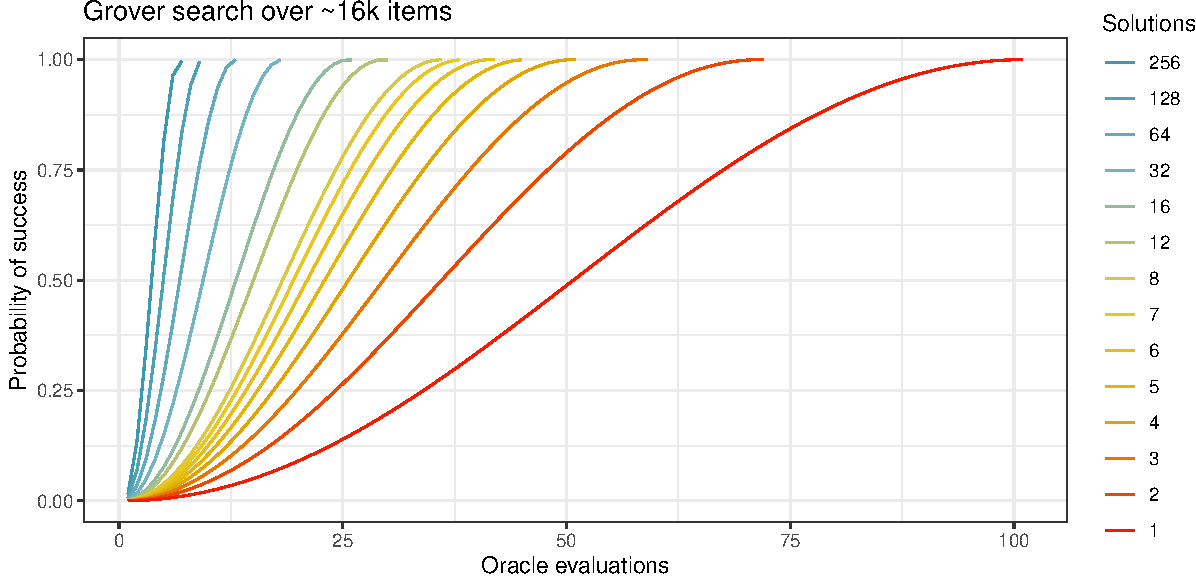
\includegraphics[width=0.9\linewidth]{groverCurves.pdf}
	\caption{Curves depict the probability that Grover's quantum search algorithm returns a solution as a function of the number of oracle evaluations. For the ranges depicted, the number of iterations required and the number of solutions inversely relate, but increasing the number of iterations past \emph{R} (Equation \ref{eq:R}) can backfire and lead to extremely small probabilities of success.  }\label{fig:grov}
\end{figure}

Given a set of $N$ items and a function $f:\{0,1,\dots,N-1\}\rightarrow \{0,1\}$ that evaluates to $1$ for a single element, \citet{grover1996fast} develops an algorithm that uses quantum parallelism to score quadratic speedups over its classical counterparts. After only $\mathcal{O}(\sqrt{N})$ evaluations of $f(\cdot)$, Grover's algorithm returns the $x\in \{0,1,\dots,N-1\}$ satisfying $f(x) =1$ with high probability.  Compare this to $\order{N}$ requirement for the randomized classical algorithm that must evaluate $f(\cdot)$ over at least $N/2$ items to obtain the same probability of detecting $x$.  The algorithm takes the state $\ket{0}^{\otimes N}\ket{1}$ as input and applies Hadamard gates to each of the individual $N+1$ input qubits.  The resulting state is 
\begin{align*}
\ket{h}\ket{-}= \left(\frac{1}{\sqrt{N}} \sum_{x=0}^{N-1} \ket{x} \right)  \frac{1}{\sqrt{2}}\left(\ket{0} -\ket{1}\right) =  \frac{1}{\sqrt{N}} \sum_{x=0}^{N-1} \ket{x} \ket{-} \, .
\end{align*}
Next, we apply the oracle gate $\U_f: \ket{x}\ket{y} \rightarrow \ket{x}\ket{y\oplus f(x)}$ and note that 
\begin{align*}
\U_f \ket{x} \ket{-} &= \U_f \ket{x} \frac{1}{\sqrt{2}}\left(\ket{0} -\ket{1}\right) 
= \frac{1}{\sqrt{2}} \big(\ket{x} \ket{0\oplus f(x)} - \ket{x}\ket{1\oplus f(x)} \big) \\
&= -1^{f(x)} \ket{x}\ket{-}  \, .
\end{align*}
Thus, $\U_f$ flips the sign for the state $\ket{x_0}$ for which $f(x_0)=1$ but leaves the other states unchanged.  If we suppress the ancillary qubit $\ket{-}$, then $\U_f$ is equivalent to the gate $\U_{x_0}$ defined as $\U_{x_0} \ket{x} = -1^{\delta_{x_0}}\ket{x}$. We may succinctly write this gate as the Householder matrix that reflects vectors about the unique hyperplane through the origin that has $\ket{x_0}$ for a normal vector:
\begin{align*}
\U_{x_0}= \I - 2 \ket{x_0}\bra{x_0} \, .
\end{align*}
The action of this gate on the state $\ket{h}$ takes the form
\begin{align*}
\frac{1}{\sqrt{N}} \sum_{x=0}^{N-1} \ket{x} \longrightarrow \frac{1}{\sqrt{N}} \sum_{x=0}^{N-1} -1^{\delta_{x_0}(x)} \ket{x} \, .
\end{align*}
Next, the algorithm reflects the current state about the hyperplane that has $\ket{h}$ as a normal vector and negates the resulting state:
\begin{align*}
\Big(2\ket{h}\bra{h}-\I \Big) \left( \frac{1}{\sqrt{N}} \sum_{x=0}^{N-1} -1^{\delta_{x_0}(x)} \ket{x}  \right)
&= \frac{1}{\sqrt{N}}\sum_{x} \left( (-1)^{1-\delta_{x_0}(x)} + 2 \frac{(N-2)}{N} \right)\ket{x}\\ &= \frac{(3N-4)}{N^{3/2}} \ket{x_0} + \sum_{x\neq x_0} \frac{(N-4)}{N^{3/2}}  \ket{x} \, .
\end{align*}
The scientist who measures the state at this moment would obtain the desired state $\ket{x_0}$ with a slightly higher probability of $(3N-4)^2/N^3$  than the individual probabilities of $(N-4)^2/N^3$ for the other states. Each additional application of the \emph{Grover iteration}
\begin{align}\label{eq:grov}
\G := - \U_h \U_{x_0} := \Big(2\ket{h}\bra{h}-\I \Big) \Big( \I - 2 \ket{x_0}\bra{x_0} \Big)
\end{align}
increases the probability of obtaining $\ket{x_0}$ at the time of measurement in the computational basis and $R=\ceil{\pi\sqrt{N}/4}$ iterations guarantees a probability of success that is greater than $1-1/N$.

  \begin{algorithm}[th!]
	\caption{Quantum exponential searching algorithm \citep{boyer1998tight}}\label{alg:expoSearch}
	\KwData{An oracle gate $\U_f$ taking $\ket{x}\ket{y}$ to $\ket{x}\ket{y\oplus f(x)}$ for a function $f(x):\{0,\dots,N-1\}\rightarrow \{0,1\}$ with unknown number of solutions; $n=\log_2(N)$.}
	\KwResult{If a solution exists, an $n$-bit binary string $x_0$ satisfying $f(x_0)=1$; if no solution exists, the algorithm runs forever.}
	$m \gets 1$\;
	$\gamma \gets 6/5$\;
	success $\gets$ \textcolor{blue}{FALSE}\;
	\While{\emph{success}$\neq$\emph{\textcolor{blue}{TRUE}}}{
		$j \gets Uniform \{0,\cdots,m-1\}$\;
		$\ket{0}^{\otimes n}\ket{1} \longrightarrow \H^{\otimes n+1}\ket{0}^{\otimes n}\ket{1}= \ket{h}\ket{-}$\; 
		$\ket{h}\ket{-} \longrightarrow \G^j \ket{h}\ket{-} = \ket{x}\ket{-}$;\hspace{1em}  \Comment{$j$ Grover iterations from Alg \ref{alg:grover}.}  
		$\ket{x} \longrightarrow x$; \hspace{16em} \Comment{Measure and check.}  
		\uIf{$f(x)=1$}{$x_0 \gets x$\;
			success $\gets$  \textcolor{blue}{TRUE}\;}
		\Else{$m \gets \min\left( \gamma m, \sqrt{N}\right)$;\hspace{4em}  \Comment{Increase $m$ in case of failure.}
	}}
	\Return{$x_0$}\ .
	
	\vspace{0.5em}
\end{algorithm}

In general, we may use Grover's search algorithm to find a solution when the number of solutions $M$ is greater than 1. While the algorithmic details change little, the number of required Grover iterations
\begin{align}\label{eq:R}
R = \ceil[\Bigg]{\frac{\pi}{4} \sqrt{\frac{N}{M}}}
\end{align}
 and the probability of success after those $R$ iterations \emph{do} change \citep{boyer1998tight}.  When $M$ is much smaller than $N$, the success rate is greater than $1-M/N$, and even for large $M$ the success rate is more than $1/2$. Lower-bounds are useful for establishing mathematical guarantees, but it is also helpful to understand the quality of algorithmic performance as a function of $M$ and $R$. Figure \ref{fig:grov} shows success curves as a function of the number of Grover iterations (or oracle calls) applied.  The search field contains $2^{14} \approx 16$k elements, and the number of solutions $M$ varies. Each curve represents an individual search task.  The algorithm requires more iterations for smaller numbers and fewer iterations for larger numbers of solutions.  The upper bound on error $M/N$ is only an upper bound: the final probability of success for, e.g., $M=256$ is 0.997 compared to the bound of 0.984.
 

 
 While Grover's algorithm delivers impressive speedups over classical search algorithms, it has a major weakness.
 Figure \ref{fig:grov} hides the fact that the probability of success for Grover's algorithm is \emph{not} monatonic in the number of iterations.  Running the algorithm for more than $R$ iterations can backfire.  For example, running the algorithm for $\sqrt{2N}$ iterations when $M=1$ results in a probability of success less than $0.095$ \citep{boyer1998tight}.  The non-monotinicity of Grover's algorithm becomes particularly problematic when we do not know the number of solutions $M$. Taking for example $N=2^{20}$, \citet{boyer1998tight} point out that 804 iterations provide an extremely high probability of success when $M=1$ but a one-in-a-million chance of success when $M=4$.  To solve this problem and develop an effective search algorithm when $M$ is unknown, those authors adopt the strategy of focusing on the expected number of iterations before success. In particular, they propose the quantum exponential search algorithm (Algorithm \ref{alg:expoSearch}).  When a solution exists, the algorithm returns a solution with expected total number of Grover iterations bounded above by $\frac{9}{2}\sqrt{N/M}$.  Still better, this upper bound reduces to $\frac{9}{4}\sqrt{N/M}$ for the special case $M\ll N$, and simulations presented in Figure \ref{fig:expo} show that even this bound is large.  Such results come in handy when deciding whether to halt the algorithm's progress if one believes it possible that no solutions exist.  Indeed, this turns out to be useful in the context of quantum minimization.
 

 
 \begin{figure}[!t]
 	\centering
 	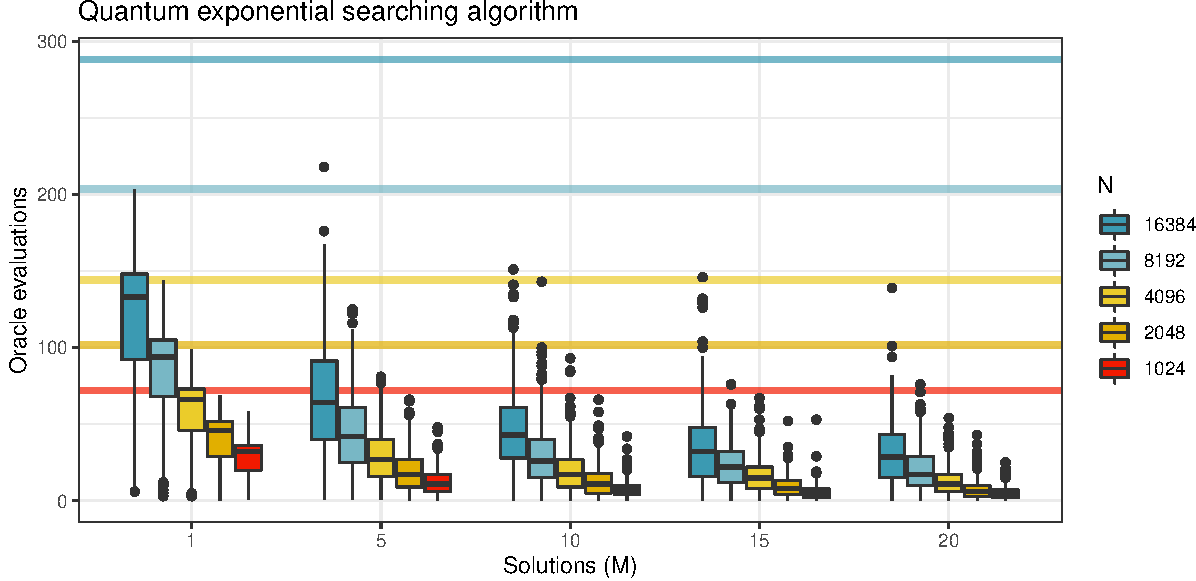
\includegraphics[width=0.9\linewidth]{expoSearch.pdf}
 	\caption{Total number of oracle evaluations required by quantum exponential searching algorithm \citep{boyer1998tight} for different numbers of solutions $M$ and search set sizes $N$ from 500 independent simulations each.  Horizontal lines at $\frac{9}{4}\sqrt{N}$ represent upper bounds on expected total number of evaluations to obtain a solution for the $M=1$ problem.}\label{fig:expo}
 \end{figure}
 

 
 \subsection{Quantum minimization}



 \begin{algorithm}[t!]
 	\vspace{3em}
 	
	\caption{Quantum minimum searching algorithm \citep{durr1996quantum}}\label{alg:min}
	\KwData{A quantum sub-routine capable of evaluating a function $f(\cdot)$ over $\{0,\dots,N-1\}$ with with unique integer values; a maximum error tolerance $\epsilon \in(0,1)$; expected total time to success $m_0=\frac{45}{4}\sqrt{N}+\frac{7}{10}\log_2(N)$.}
	\KwResult{A $\log_2 (N)$-bit binary string $x_0$ satisfying $f(x_0) = \min f$ with probability greater than $1-\epsilon$.}
	$s \gets 0$\;
	$x_0 \gets Uniform\{0,\dots,N-1\}$\;
	\While{$s< m_0/\epsilon$}{
		Prepare initial state $\frac{1}{\sqrt{N}}\sum_x\ket{x}\ket{x_0}$\;
		Mark all items $x$ satisfying $f(x)<f(x_0)$\;
		$s\gets s+ \log_2(N)$\;
		Apply quantum exponential searching algorithm (Alg \ref{alg:expoSearch}); \Comment{$I$ time steps}
		$s\gets s+ I$\;
		Obtain $x'$ by measuring first register\;
		\If{$f(x')<f(x_0)$}{$x_0 \gets x'$}
	}
	\Return{$x_0$} \ .
	\vspace{0.5em}
	
\end{algorithm}
		


Given a function $f(\cdot)$ that maps the discrete set $\{0,\dots,N-1\}$ to the integers, we wish to find the minimizer
\begin{align*}
x_0 = \argmin_{x\in\{0,\dots,N-1\}} f(x) \, .
\end{align*}
 \citet{durr1996quantum} propose a quantum algorithm for finding $x_0$ that iterates between updating a running minimum $F\in f(\{0,\dots,N-1\})$ and applying the quantum exponential search algorithm (Algorithm \ref{alg:expoSearch}) to find an element $x$ such that $f(x)<F$.  Having run these iterations a set number of times, the algorithm returns the minimizer $x_0$ with high probability. 
 To this end, \citet{durr1996quantum} show that their algorithm takes an expected total time less than or equal to $m_0:=\frac{45}{4}\sqrt{N}+\frac{7}{10}\log_2(N)$ to find the minimizer, where marking items with values less than the threshold value (Algorithm \ref{alg:min}) requires $\log_2(N)$ time steps and each Grover iteration within the quantum exponential search algorithm requires one time step. From there, Markov's inequality says
 \begin{align*}
 \mbox{Pr}\left( \mbox{total time to success} \geq \frac{m_0}{\epsilon}\right) \leq \frac{\mbox{E}\left(\mbox{total time to success}\right)}{m_0/\epsilon}\leq \epsilon \, ,
 \end{align*}
 or that we must scale the minimization procedure's time steps by a factor of $1/\epsilon$ to reach a failure rate less than $\epsilon$.  Due to the iterative nature of the algorithm, one might suppose that it is beneficial to start at a value $x_0$ for which $f(x_0)$ is lower relative to other values. This turns out to be the case in theory and in practice, and the benefit of warm-starting is particularly useful in the context of parallel MCMC.



\begin{prop}[Warm-starting]\label{prop:warm}
	Suppose that the quantum minimization algorithm begins with a threshold $F_0$ such that $f(x)<F_0$ for only $K-1$ items. Then the expected total number of time steps to find the minimizer is bounded above by
	\begin{align*}
	m_0^K = \left(\frac{5}{4} - \frac{1}{\sqrt{K-1}} \right) 9\sqrt{N} + \frac{7}{10} \log_2(K) \log_2(N) \, ,
	\end{align*}
	and so the following rule relates the warm-started upper bound to the generic upper bound:
	\begin{align*}
	m_0^K = m_0 - 9\sqrt{\frac{N}{K-1}} + \frac{7}{10} \log_2 \left(\frac{K}{N} \right) \log_2(N)\, .
	\end{align*} 
\end{prop}

\begin{proof}
	The proof follows the exact same form as Lemma 2 of \citet{durr1996quantum}. It relies on a theoretical algorithm called the \emph{infinite algorithm} that runs until the minimum is found.  In this case, Lemma 1 of that paper says that the probability that the $r$th lowest value is ever selected when searching among $K$ items is $p(K,r)=1/r$ for $r\leq K$ and 0 otherwise.  For a warm-start at element $K$, the expected total time spent in the exponential search algorithm is
	\begin{align*}
	\sum_{r=2}^N p(K,r) \frac{9}{2} \sqrt{\frac{N}{r-1}} &= \sum_{r=2}^K p(K,r) \frac{9}{2} \sqrt{\frac{N}{r-1}} 
	=  \frac{9}{2}\sqrt{N}\sum_{r=1}^{K-1} \frac{1}{r+1} \frac{1}{\sqrt{r}} \\
	&\leq \frac{9}{2}\sqrt{N}\left( \frac{1}{2}+\sum_{r=2}^{K-1} r^{-3/2} \right) \leq \frac{9}{2}\sqrt{N}\left( \frac{1}{2}+\int_{r=1}^{K-1} r^{-3/2} \dd r \right) \\
	&= \left(\frac{5}{4} - \frac{1}{\sqrt{K-1}} \right) 9\sqrt{N} \, .
	\end{align*}
	An upper bound for the expected total number of time steps preparing the initial state and marking items $f(x)<f(x_0)$ follows in a similar manner.
\end{proof}



Proposition \ref{prop:warm} shows that, e.g., if Algorithm \ref{alg:min} begins at the item with second lowest value, then the expected total time to success is bounded above by $m_0^2=\frac{9}{4}\sqrt{N}+\frac{7}{10}\log_2(N)$, reducing the generic upper bound by $9\sqrt{N}-\frac{7}{10}\log_2\left( \frac{2}{N}\right)\log_2(N)$ time steps.  When $N$ equals 1000, say, the expected total time steps is $m_0^2< 78.2$.  Keeping $N=1000$ but letting the algorithm begin at the third lowest value ($K=3$), the expected total time steps before success is $m_0^3<165.6$. Raising $N$ to 10,000, the two numbers increase to $m_0^2< 234.4$ and $m_0^3<503.4$.  

In practice, the number of time steps before finding the minimum is surprisingly small.  Figure \ref{fig:qMinAlg} corroborates the intuition that it is beneficial to start at a lower ranked element. To generate these results, we use an early stopping rule for the quantum minimization algorithm's exponential searching sub-routine, halting it after $\frac{9}{4}\sqrt{N}$ iterations. Even with this stopping rule in place, the error rate of the quantum minimization algorithm is less than $1\%$. We can increase the early stopping threshold to obtain even lower error rates, but this strategy would seem to be unnecessary in the context of parallel MCMC.  The benefits of warm-starting are useful in the same context, when the current state $\ttheta^{(s)}$ usually inhabits the high-density region of the target distribution but the majority of proposals do not.  

 \begin{figure}[!t]
	\centering
	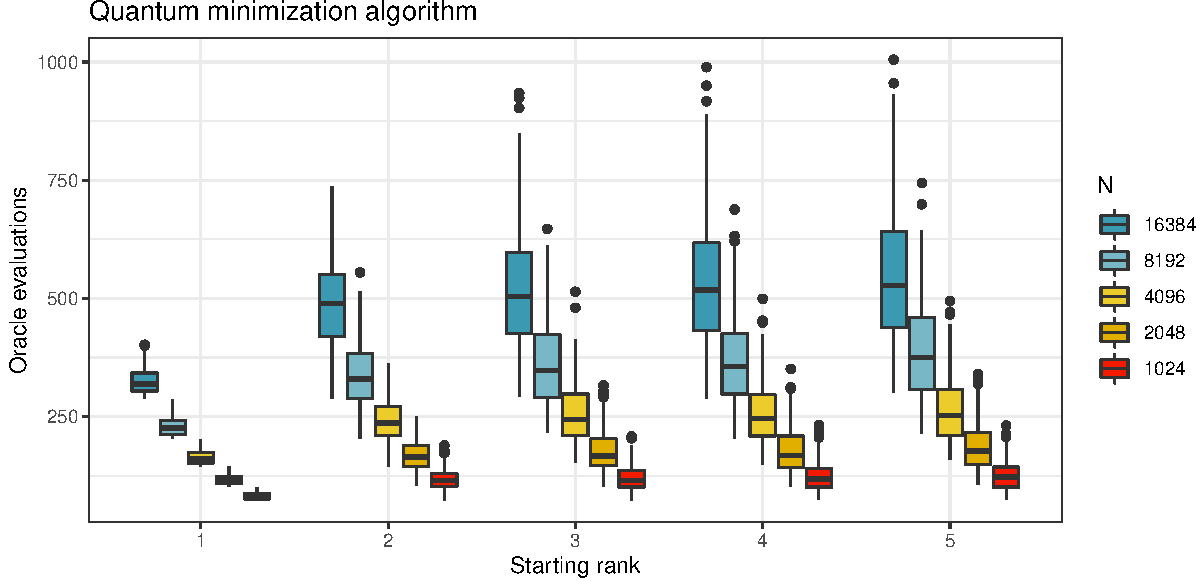
\includegraphics[width=0.9\linewidth]{qMinAlg.pdf}
	\caption{Total number of oracle evaluations required by quantum minimization algorithm \citep{durr1996quantum} for different starting ranks and search set sizes $N$ from 500 independent simulations each.  Here, less than 1\% of the 12,500 instances fail to recover the true minimum on account of early stopping.}\label{fig:qMinAlg}
\end{figure}

\section{Quantum parallel MCMC}

With the rudiments of quantum minimization in hand, we present a quantum parallel MCMC (QPMCMC). The general structure of the algorithm the same as Algorithm \ref{alg:pMCMC}: it constructs a Markov chain by iterating between generating many proposals and randomly selecting new Markov chain states among these proposals.  Unlike classical single-proposal MCMC, parallel MCMC proposes many states and chooses one according to the generalized acceptance probabilities of Equation \eqref{eq:probs}.
 In general MCMC, evaluation of the target density function $\pi(\cdot)$ is the rate-limiting computational step, becoming particularly onerous in big data scenarios \citep{massive}.  While parallel MCMC benefits from improved mixing as a function of MCMC iterations, the increased computational burden of $P$ target evaluations at each step can lead to less favorable comparisons when accounting for elapsed wall-clock time.
 
 \emph{Having successfully generated proposals $\ttheta_p,$ $p=1,\dots,P$ and evaluated the corresponding proposal densities $q(\cdot,\cdot)$, we would like to use quantum parallelism and an appropriate oracle gate to efficiently compute the $\pi(\ttheta_p)$s but immediately encounter a Catch-22 when we seek to draw a sample $\ttheta^{(s+1)} \sim$ \emph{Discrete}$(\ppi)$ for $\ppi$ the vector of probabilities $\pi_0,\pi_1,\dots,\pi_P$ defined in Equation \eqref{eq:probs}.  We can use neither a quantum nor a classical circuit to draw the sample! On the one hand, drawing the sample within a quantum circuit would somehow require that all superposed states have access to all the $\pi(\ttheta_p)$s at once to perform the required normalization.  On the other hand, drawing the sample within the classical circuit would require access to all the $\pi(\ttheta_p)$s, but measurement in the computational basis can only return one.}  
 
 In light of this dilemma, we propose to use the Gumbel-max trick \citep{papandreou2011perturb} to transform the generalized accept-reject step into a discrete optimization procedure.  From there, we use quantum minimization to efficiently sample from $Discrete(\ppi)$. Crucially, we get away with quantum parallel evaluation of the target $\pi(\cdot)$ over all superposed states because the Gumbel-max trick does not rely on a normalization step: each superposed state requires no knowledge of any target evaluation other than its own.  

\subsection{Gumbel-max}\label{sec:gm}
\newcommand{\p}{\mbox{p}}

\begin{algorithm}[!t]
	\caption{The Gumbel-max trick}\label{alg:gm}
	\KwData{A vector of unnormalized log-probabilities $\llambda^*=\log \ppi +\log c$, for $\ppi$ a discrete probability vector with $P+1$ elements.}
	\KwResult{A single sample $p \sim$ \emph{Discrete}$(\ppi)$ satisfying $p\in\{0,1,\dots,P\}$.}
	\For{$p' \in\{0,1,\dots,P\}$}{
		$z_{p'} \gets Gumbel(0,1)$\;
		$\alpha^*_{p'} \gets \lambda_{p'}^* + z_{p'}$\;
	}
	$p \gets \argmax_{p'=0,\dots,P}\alpha^*_{p'}$\;
	\Return{p}\ .
	
	\vspace{0.5em}
\end{algorithm}

We wish to randomly select a single element from the set $\{0,1,\dots,P\}$ with probability proportional to the unnormalized probabilities $\ppi^*=(\pi_0^*,\pi_1^*,\dots,\pi_P^*)$.  That is, there exists a $c>0$ such that $\ppi^* = c \ppi$, for $\ppi$ a valid probability vector, but we only have access to $\ppi^*$.  Define $\llambda:= \log \ppi$ and $\llambda^*:= \log \ppi^*=\log\ppi + \log c$,  and assume that $z_0,\dots,z_P\stackrel{iid}{\sim}Gumbel(0,1)$. Then, the probability density function $g(\cdot)$ and cumulative distribution function $G(\cdot)$ for each individual $z_p$ are
\begin{align*}
g(z_p) = \exp\big(-z_p- \exp(-z_p)\big)  \quad \mbox{and} \quad G(z_p) = \exp \big( -\exp(-z_p) \big)\, .
\end{align*}
Now, defining the random variables $\alpha^*_p:=\lambda^*_p+z_p$, $\alpha_p:=\lambda_p+z_p$ and  
\begin{align*}
\hat{p} = \argmax_{p=0,\dots,P}\: \alpha^*_p \, ,
\end{align*}
we have the result
\begin{align*}
\mbox{Pr} (\hat{p} = p) = \pi_p \, .
\end{align*}
In words, the procedure of adding Gumbel noise to unnormalized log-probabilities and taking the index of the maximum produces a random variable that follows the discrete distribution over $\ppi$.  Moving from left to right:
\begin{align*}
\mbox{Pr} (\hat{p} = p) &= \mbox{Pr} (\alpha^*_p > \alpha^*_{p'}, \, \forall p' \neq p ) \\
&= \mbox{Pr} (\alpha_p +\log c > \alpha_{p'} + \log c, \, \forall p' \neq p ) 
= \mbox{Pr} (\alpha_p  > \alpha_{p'} , \, \forall p' \neq p ) \\
&= \int_{-\infty}^\infty \prod_{p'\neq p} \mbox{Pr} (\alpha_p > \alpha_{p'}| \alpha_p) g(\alpha_p-\lambda_p) \, \dd \alpha_p 
= \int_{-\infty}^\infty \prod_{p'\neq p} G(\alpha_p-\lambda_{p'}) g(\alpha_p-\lambda_p) \, \dd \alpha_p \\
&=  \int_{-\infty}^\infty  \prod_{p'\neq p} \exp\big( -\exp(\lambda_{p'}-\alpha_p)\big) \exp\big(-\alpha_p+\lambda_p - \exp(-\alpha_p+\lambda_p) \big) \, \dd \alpha_p \, .
\end{align*}
Recalling that $\lambda_{p'}=\log \pi_{p'}$, we exponentiate the logarithms, and the integral becomes
\begin{align*}
& \pi_p \int_{-\infty}^\infty  \prod_{p'\neq p} \exp\big( -\pi_{p'}\exp(-\alpha_p)\big) \exp  \big(-\alpha_p - \pi_p\exp(-\alpha_p) \big) \, \dd \alpha_p \\
&= \pi_p \int_{-\infty}^\infty \exp  (-\alpha_p ) \exp\big( -\sum_{p'=0}^P\pi_{p'}\exp(-\alpha_p)\big)  \, \dd \alpha_p  \\
&= \pi_p \int_{-\infty}^\infty \exp  (-\alpha_p ) \exp\big( -\exp(-\alpha_p)\big)  \, \dd \alpha_p  = \pi_p \, ,
\end{align*}
where the final equality follows easily from a change of variables.  QPMCMC combines this trick with the quantum minimization algorithm presented in Section \ref{sec:qmin}.





\subsection{QPMCMC}

\begin{algorithm}[t!]
	\caption{Quantum parallel MCMC}\label{alg:qpMCMC}
	\KwData{Initial Markov chain state $\ttheta^{(0)}$; total length of Markov chain $S$; total number of proposals per iteration $P$; routine for evaluating target density $\pi(\cdot)$; routines for drawing random samples from the proposal distribution $Q(\ttheta^{(s)},\cdot)$ and the standard Gumbel distribution $Gumbel(0,1)$.}
	\KwResult{A Markov chain $\ttheta^{(1)}, \dots, \ttheta^{(S)}$.}
	\For{$s \in\{1,\dots,S\}$}{
		%$\sigma_\pi \gets 0$\;
		$\ttheta_0 \gets \ttheta^{(s-1)}$\;
		\For{$p' \in \{1,\dots,P\}$}{
			$\ttheta_{p'} \gets Q(\ttheta^{(s-1)},\cdot)$\;
		}
		\For{$p' \in \{0,\dots,P\}$}{
			$q_{p'} \gets  \prod_{p''\neq p'}q(\ttheta_{p'},\ttheta_{p''})$\; 
			$z_{p'} \gets Gumbel(0,1)$\;
		}
		$p \gets \argmin_{p'=0,\dots,P}f(p')= -\left(\log \big(\pi(\ttheta_{p'}) q_{p'}\big) + z_{p'}\right)$; \hspace{2em} \Comment{$\order{\sqrt{P}}$ Alg \ref{alg:min}}
		$\ttheta^{(s)} \gets \ttheta_p$\;
	}
	\Return{$\ttheta^{(1)}, \dots, \ttheta^{(S)}$}\ .
	
	\vspace{0.5em}
\end{algorithm}

 \begin{figure}[!t]
 	\vspace{3em}
	\centering
	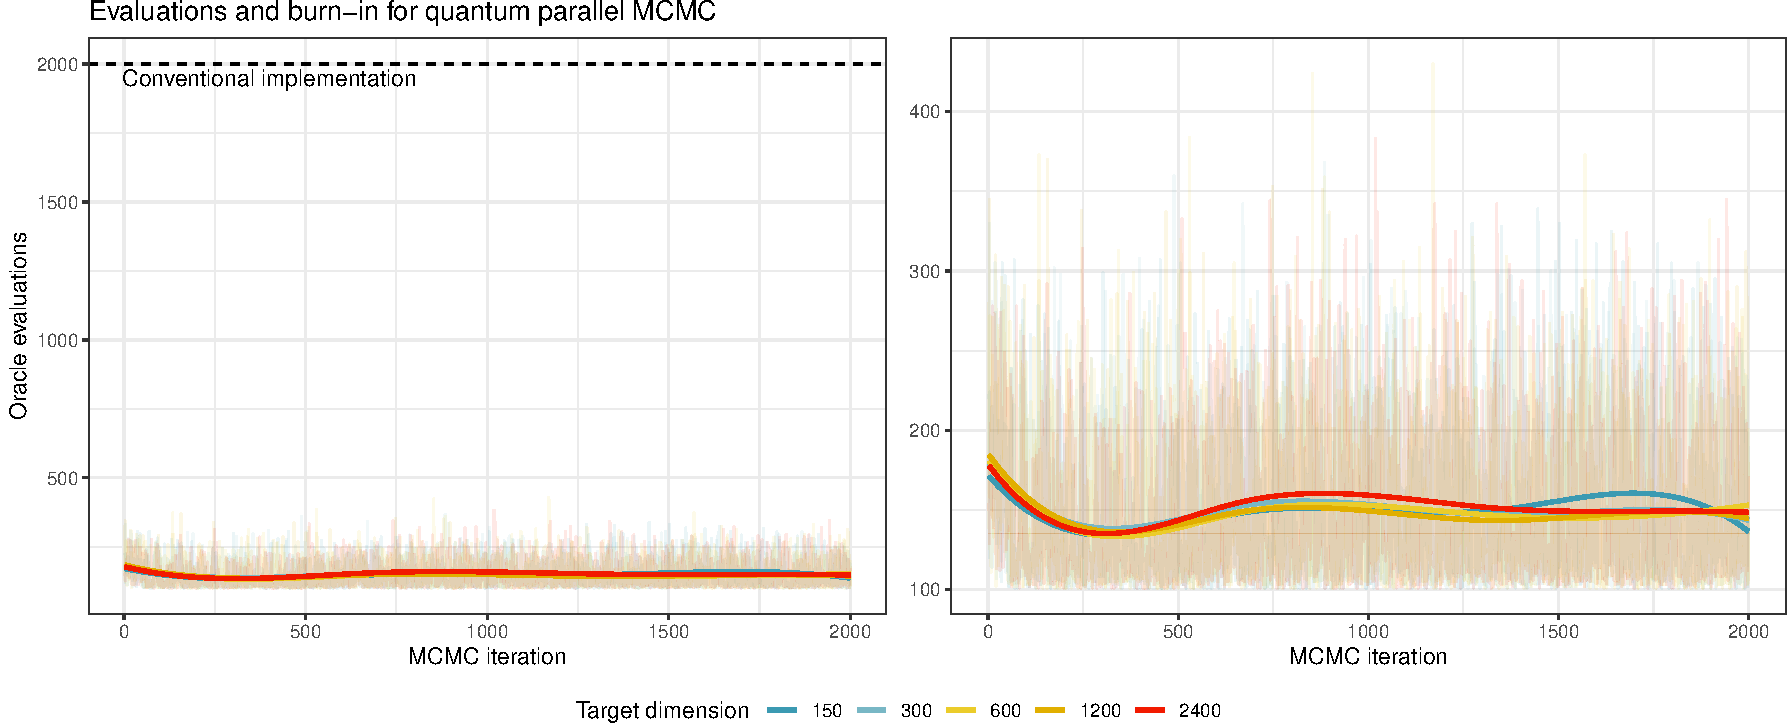
\includegraphics[width=0.9\linewidth]{mcmcIterations.pdf}
	\caption{Total number of oracle evaluations required for each of 2,000 parallel MCMC iterations. In total, the combined MCMC runs required roughly $7$\% of the usual 20 million target evaluations. Over  99.4\% of the 10,000 MCMC iterations successfully sampled from the discrete distribution with probabilities of Equation \eqref{eq:probs}. Burn-in evaluations require moderately more evaluations because the current state occupies a lower density region and represents a `less good' warm-start.}\label{fig:mcmcIterations}
\end{figure}




 \begin{figure}[ph!]
	\centering
	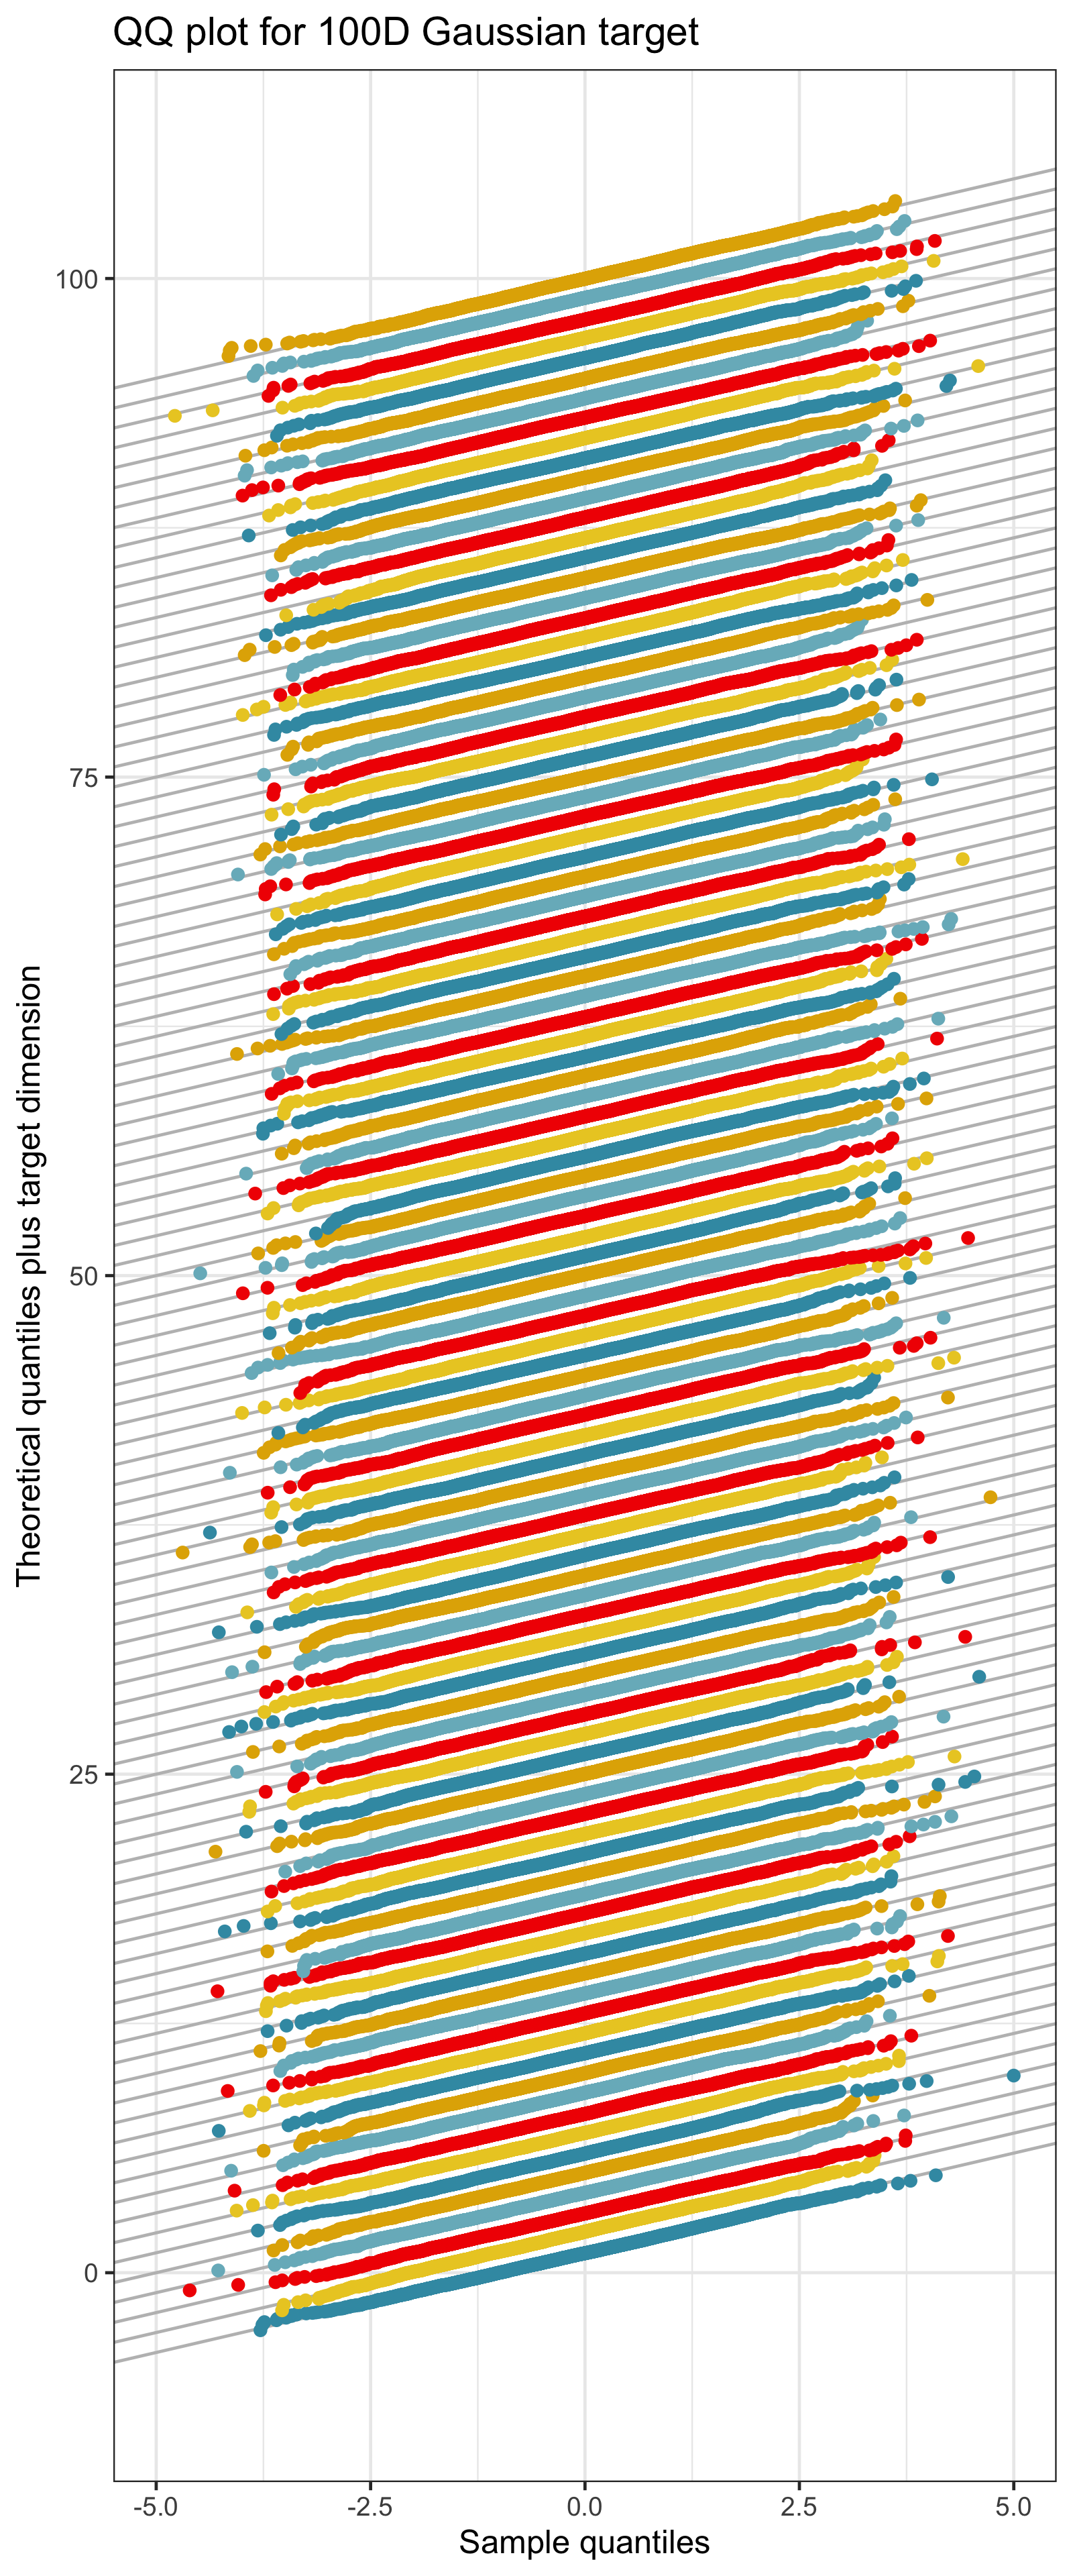
\includegraphics[width=0.5\linewidth]{qqPlot.png}
	\caption{Empirical accuracy of quantum parallel MCMC (QPMCMC) for a 100 dimensional spherical Gaussian target.  We generate 100,000 samples using 2,000 proposals each iteration and remove the first 2,000 samples as burn-in.  The QQ (quantile-quantile) plot shows sample quantiles adhering closely to the theoretical quantiles.  Similar to the independent simulation shown in Figure \ref{fig:mcmcIterations}, here QPMCMC requires less than $7.2$\% of the usual number of target evaluations.}\label{fig:qq}
\end{figure}

Algorithm \ref{alg:qpMCMC} presents the details of QPMCMC.  The algorithm uses conventional (perhaps parallel) computing almost entirely, excluding the one line that calls the quantum minimization algorithm presented in Algorithm \ref{alg:min}. This sub-routine seeks to find the minimizer of the function
\begin{align*}
f(p')= -\left(\log \big(\pi(\ttheta_{p'}) q_{p'}\big) + z_{p'}\right) \quad \mbox{over} \quad p'=0,1,\dots, P,
\end{align*} 
which combines the numerators of Equation \eqref{eq:probs}, the Gumbel-max trick and a trivial negation.  As discussed in Section \ref{sec:qmin}, the sub-routine requires only $\mathcal{O}(\sqrt{P})$ oracle evaluations and, therefore, only $\mathcal{O}(\sqrt{P})$ evaluations of the target density $\pi(\cdot)$ using a quantum circuit.  In theory, a quantum computer can perform the same computations as a classical computer, but the efficiency of the target evaluations would depend on a number of factors related to the structure of the density itself, the availability of fast quantum random access memory \citep{giovannetti2008quantum} and the ability of large numbers of quantum gates to act in concert with negligible noise \citep{kielpinski2002architecture,erhard2019characterizing}.

In general MCMC, one often calibrates the scaling of a proposal kernel to balance between exploring the target's domain and remaining within high-density regions.  Optimal scaling strategies may lead to a large number of rejected proposals \citep{roberts2001optimal}.  Indeed, \citet{holbrook2021generating} shows that parallel MCMC algorithms are no exception. When using the Gumbel-max trick to sample from proposals, this means that the current state is often quite near optimality, representing a warm-start.  Figure \ref{fig:mcmcIterations} shows how this warm-starting effects the number of oracle calls (and hence target evaluations) within the quantum minimization sub-routine over the course of an MCMC trajectory.  We target multi-dimensional standard normal distributions of differing dimensions using the vector $(100,\dots,100)$ as starting position. We fix the number of Gaussian proposals to be 2,000 and use standard adaptation procedures to target a 50\% acceptance rate while guaranteeing convergence \citep{rosenthal2011optimal}. Across iterations, QPMCMC requires relatively few oracle calls compared to the 2,000 target evaluations of parallel MCMC. We also witness the expected drop in the number of oracle evaluations as the chain approaches the target's high-density region. Remarkably, the algorithm succeeds in sampling from the true discrete distribution in 99.5\% of the MCMC iterations. An independent simulation obtains similar results, requiring roughly 7\% of the usual number of target evaluations. Figure \ref{fig:qq} shows a quantile-quantile plot for all 100 dimensions of a multi-dimensional standard normal distribution. We see no appreciable impact from the rare failure of the quantum minimization sub-routine.

%\begin{table}[ht]\centering
%	\begin{tabular}{llll}  \toprule 
%	Proposals	& Effective samples (ES) & Evaluations per ES & Speedup \\   \midrule
%	1 (MH)	 & 21.35  (11.74, 50.65) & 429.81  (180.15, 766.89) & 1.00  (1.00, 1.00) \\  
%		 50 & 736.25 (418.73, 1072.35) & 259.54  (177.72, 475.16) & 1.66  (1.01, 1.61) \\  
%		 100 & 1842.71 (1604.07, 2097.74) & 146.49  (128.76, 168.39) & 2.93 (1.40, 4.55) \\  
%		 150 & 2287.03  (1734.34, 2444.05) & 146.39 (137.36, 193.16) & 2.94 (1.31, 3.97) \\ 
%		  200 & 2662.89  (2547.71, 2844.14) & 145.92 (136.37, 152.74) & 2.95  (1.32, 5.02) \\ 
%		   250 & 2971.59  (2439.45, 3208.46) & 147.77  (136.53, 180.95) & 2.91  (1.32, 4.24) \\  
%		  \bottomrule\end{tabular}
%\end{table}

\subsection{Note on simulations}

We use the \textsc{R} programming language \citep{rlang} for all simulations and the \textsc{ggplot2} package to generate all figures \citep{ggplot}.  All simulations rely on the fact that the Grover iterations of Equation \eqref{eq:grov} manipulate the probability amplitudes in a deterministic manner. For example, the following \textsc{R} code specifies $N$ uniform probability amplitudes (\verb|sqrtProbs|), performs $I$ Grover iterations and measures a single state according to the resulting probabilities.
\begin{minted}{R}
sqrtProbs <- rep(1/sqrt(N),N); i <- 1
while (i <= I) {
	sqrtProbs  <- -marks*sqrtProbs + (1-marks)*sqrtProbs
	sqrtProbs  <- -sqrtProbs + 2*mean(sqrtProbs)
	i <- i + 1
}
measurement <- sample(size=1, x=1:N, prob=sqrtProbs^2)
\end{minted}
Of course, simulating these iterations on a classical computer, requires precomputing the values of \verb|marks| beforehand.


\section{Discussion}

We have shown how parallel MCMC may enjoy quadratic speedups by combining quantum minimization with the Gumbel-max trick.  Within a QPMCMC iteration, the current state represents a warm-start for the sampling-turned-optimization problem, leading to increased efficiencies for the quantum minimization algorithm.  This work leads to two immediate questions.  First, more recent quantum minimization algorithms exist \citep{baritompa2005grover,farhi2014quantum}.  Would these confer additional speedups for quantum parallel MCMC and benefit from warm-starting in a similar manner? Second, there are other algorithms in statistics and machine learning that require sampling from potentially costly discrete distributions \citep{liu2001theoretical,csillery2010approximate}.  Can one adapt  the proposed strategies to these?  Large-scale, practical quantum computing is still a long way off, but quantum algorithms are ripe for conventional computational statistics.

\bibliographystyle{sysbio}
\bibliography{refs}

\appendix




%%%%%%%%%%%%%%%%%%%%%%%%%%%%%%%%%%%%%%%%%%%%%%%%%%%%%%%%%%%%

\end{document}


\centerline{\large \bf Reponse to Editor and Reviewer Comments}

To the Editors and Reviewers:

I appreciate the thoughtful comments and recommendations made by the AE and Reviewers and the opportunity to revise my manuscript ``\paperTitle" (\paperID).
I have carefully considered these extremely helpful suggestions and have addressed them to the best of my abilities.  I believe that the manuscript is now significantly improved and am thankful for the time and energy put forth by the Editors and Reviewers.

In particular, I have:
\begin{itemize}
	\item done things
\end{itemize}


The document below contains my replies (in \textbf{bold}) alongside the AE and Reviewers' comments (normal text).  I list changes to the text with indented normal text set off by quotation marks.

With sincere gratitude,

Andrew Holbrook
\clearpage


{\Large \bf Editor and Reviewer Comments:}


\section*{Reviewer 1}


This paper presented an interesting framework for large-scale MCMC. It leverages the quantum speedup of Grover's searching algorithm to accelerate the treatment of multi-proposals in MCMC. However, an implementation of a quantum algorithm involves nontrivial steps, which need to be explained before this paper can be accepted.

The author did not clarify whether this is a fully quantum algorithm, or a hybrid one. It is important to explain what is the input of the quantum computer and what to extract. For the input, one has to encode it coherently into a quantum state $\ket{\psi}$, and estimate the complexity associated with such preparation.

To extract quantities from a quantum computer, one has to express it as an expectation (observable), and estimate the probability of obtaining the correct output. 

There have already been numerous quantum algorithms for MCMC, e.g.,
\begin{enumerate}
	\item Montanaro, A. Quantum Speedup of Monte Carlo Methods. Proc. R. Soc. A. 2015, 471 (2181), 20150301. \citep{montanaro}
	
	\item Wocjan, P.; Abeyesinghe, A. Speedup via Quantum Sampling. Phys. Rev. A 2008, 78 (4), 042336. \citep{wocjan2008speedup}
\end{enumerate}
The author should comment on how the present approach would compare to these existing methods.


\section*{Reviewer 2}


This paper seeks to further develop parallel Markov chain Monte Carlo in the quantum computing hardware. The topic is very interesting. The author has a nice comprehensive review of multi-proposal parallel MCMC, and is very current in literature. The review of established quantum computing algorithms is also very helpful for statistician who might have limited knowledge in the area. 

The key contribution is connecting parallel Markov chain Monte Carlo to the quantum computing. The key step is to employ Gumbel-max trick to transform the generalized accept-reject step (i.e., Dirichlet sampling) into a discrete optimization procedure, so that quantum optimization algorithm can be used for sampling. The idea is simple and elegant. It just connects the dots.

I still have a few concerns, more generally related to the “bedrock” parallel Markov chain Monte Carlo:

\begin{enumerate}
	\item Although named as parallel MCMC, the algorithm is still MCMC, which relies on the back-bone Markov chain to achieve equilibrium. The algorithm still heavily relies on the long sequence for the Markov chain to reach equilibrium. The quantum part doesn’t seem to be able to solve this major drawback of parallel MCMC. 
	
	\item I see more potential of the Gumbel-max trick $+$ quantum computing in sequential Monte Carlo. Unlike MCMC, SMC only requires a handful of sequential chains, and mostly need to have a very large number of proposals for re-sampling, where your trick could have more impact.
	
	\item A last comment is on computer hardware structure. In the QPMCMC, the Markov chain for loop requires CPU, the evaluation of log-likelihood requires GPU, and the sample from Dirichlet requires quantum processor. Will there be I/O communication overhead for these steps on distinct processors?
\end{enumerate}






\section*{Associate Editor}



The author proposes a quantum parallel MCMC algorithm that uses a Gumbel-max trick to quantum parallelize a multiple-proposal MCMC algorithm. The resulting algorithm drastically reduces the number evaluations of the target density. The manuscript is quite well written and motivated.


The referees are relatively positive about the work, however, certain improvements are deemed necessary and the points raised by them are important. I highlight a few points here, and have some additional comments.


The first referee highlights that more specific details about the quantum algorithm are required. The second referee asks an important question regarding the cost of the I/O communication. I would further add that in the displayed Algorithms, it would be useful to indicate which components are CPU parallelized, GPU parallelized, and quantum parallelized.


The author has motivated the need for quantum algorithms for big-data problems where evaluation of the target is expensive. However, only data-less examples have been implemented. Implementation on a real example is warranted. Further, comparisons with other quantum methods (as suggested by referee) would be useful to understand the effectiveness of the proposed methodology. Finally, comparison with the non-quantum version of the multiple-proposal would be helpful to make the point that the mixing of the algorithm remains unaffected.

\subsection*{Additional Comments}


\begin{itemize}
	\item (I am assuming the following is true.) It would be helpful to state clearly at some point that the resulting QPMCMC chain has the same transition kernel as the non-quantum version. That is, it remains exact.
	
	\item Equation (1): It is not clear to me how the ``a.s.'' applies to this definition of 1
	stationarity.
	
	\item Algorithm 1: The algorithm of Tjelmeland (2004) is described here as ``Parallel MCMC'', but it is not immediately clear which part of the algorithm will be implemented in a parallelizable way. I would recommend changing the caption.
	
	\item page 4, line 10: I believe the citation for \citet{gelman1992inference} is incorrect. Did the author mean \citet{gelman1992inference}?
	
	\item Algorithm 5: Should the last step be ``return $\hat{p}$''.
	
	\item Section 3.1: The proof of the Gumbel-max trick can likely be either removed or
	moved to the Appendix, since this is a fairly well-known result.
	
	\item Algorithm 6: I would recommend explicitly highlighting which parts of this algorithm are quantum parallelized.
	
	\item Figure 5: The caption here is confusing. It reads ``Total number of oracle evaluations required for each of 2000 parallel MCMC iterations''. Traditionally, this would imply there were 2000 independent chains runs. However, the text describing this Figure implies that there were 2000 Gaussian proposals.
	
	\item page 22: The authors tune to 50\% acceptance rate, but I believe the optimal in high- dimensions from the reference \citet{rosenthal2011optimal} is 23.4\%. Further, the tuning to 23.4\% acceptance rate is strictly for the Metropolis-Hastings acceptance function. In the multiple-proposal world, the acceptance function employed is completely different, implying different optimality results. See \citet{agrawal2021optimal}.
	
	
	\item Figure 5: ``Over 99.4\% of the 10,000 MCMC iterations successfully sampled from the discrete distribution with probabilities of Equation (2)''. It’s unclear exactly how this number comes about and what it means. Once the quantum minimization returns a $\hat{p}$, the authors have shown that it follows the right distribution. How can then (1) .6\% not be from the right distribution, and (2) how does one even quantify this.
	
	\item Figure 6: Considering the target is known, burn-in seems incredibly wasteful. Once can just start from stationarity and remove the need to throw away samples.
	
	\item Table 1: In producing this table, what effective sample size is being used for this two-dimensional problem?
	
	\item Could the authors comment on the potential applicability of the algorithm on discrete state spaces? This may be useful for Bayesian record linkage, and variable selection problems \citep{zanella2020informed}.
	
	
\end{itemize}


%\section{Reviewer 1}
%
%
%The author introduces \emph{simplicial samplers}, which are Markov chain Monte Carlo (MCMC) methods that sample multiple proposals at each iteration by randomly rotating a simplex and randomly
%selecting a proposal among those produced. After reading the paper a couple of times, I understood
%that it contributes to the literature. It was not clear at the beginning because the way the paper is
%written is often opaque and not detailed enough. Also, even if the paper contributes to the literature, to me, the contribution is not significant enough at the moment. In the light of the above, the
%paper cannot be accepted as is, but could be after a major revision.
%
%I will now state what is the main contribution of the paper (at least from what I understood).
%The main contribution is: within the framework of \citet{tjelmeland2004using}, to introduce a proposal
%scheme which is effective and satisfies the condition mentioned in Proposition 1, thus leading to
%MCMC methods which sample and use multiple proposals at each iteration while not requiring the
%typical accept/reject step. With this sampler, there is a positive probability of staying at the same
%state because the current state is among the proposals, but the design of the proposal scheme is
%such that, by itself, it allows to satisfy detailed balance. From the algorithm presented in Section
%3, it seems that in general the probability of leaving the current state increases with the number of
%proposals. The author may want to highlight all that and how the proposed samplers contrast with
%other relevant samplers.
%
%To me, the proposed samplers are strongly connected to multiple-try Metropolis (MTM) \citep{liu2000multiple} and that connection is not sufficiently exploited (in fact, it is not even mentioned). The
%connection becomes clear to me in Section 3.1.1 when the author describes the Gaussian variant of
%the proposed samplers. Let $\TTheta$ be the current state of the Markov chain. The author writes in that
%section: each of the proposals has a Gaussian marginal distribution with mean $\TTheta$ and covariance
%matrix $\lambda^2\mathbf{I}$ and one proposal, say $\TTheta^*$, will be randomly selected for the next state of the chain with
%probability proportional to $\pi(\TTheta^*)$ where $\pi$ is the target density. MTM works very similarly. MTM is
%one of the most popular samplers that can make effective use of parallel computing. The author could
%therefore contrast the algorithms with MTM so that we understand the similarities and differences.
%It would help to understand why and when they are expected to be better. The proposed samplers
%for instance require the sampling of a random rotation which seems to be computationally costly.
%
%	\renewcommand{\x}{\mathbf{x}}
%\renewcommand{\v}{\mathbf{v}}
%\renewcommand{\TTheta}{\boldsymbol{\theta}}
%\renewcommand{\TTTheta}{\boldsymbol{\Theta}}
%\renewcommand{\tr}{\mbox{tr}}
%\renewcommand{\X}{\mathbf{X}}
%\renewcommand{\u}{\mathbf{u}}
%\newcommand{\QQ}{\mathbf{Q}}
%\newcommand{\haar}{\mathcal{H}}
%\newcommand{\orthog}{\mathcal{O}}
%\newcommand{\SSigma}{\boldsymbol{\Sigma}}
%\newcommand{\dd}{\mbox{d}}
%
%\begin{reply}
%	We thank the Reviewer for taking the time to review our manuscript and now recognize that the previous version was opaque and that MTM did not feature prominently enough.  To address this, we have completely rewritten the introduction using MTM as our starting point and carefully provided reasons we are interested in exploring other multiproposal algorithms. These are the first two paragraphs of the introduction:
%	\begin{quote}
%		Generating random samples from probability distributions is a crucial task in many of the quantitative sciences. Markov chain Monte Carlo (MCMC) algorithms sample from target distributions by constructing Markov chains that maintain their targets as equilibrium distributions. The classic Metropolis-Hastings (MH) algorithm \citep{metropolis1953equation,hastings1970monte} builds such a Markov chain by iteratively generating a single proposal state conditioned on the current state and randomly accepting or rejecting that proposal based on a ratio involving the target and proposal densities evaluated at the current and proposed states.  The majority of MCMC techniques share this general structure, randomly proposing and accepting a single proposal at each iteration, but some relatively recent methods make use of multiple proposals (or, \emph{multiproposals}) at each step with the goals of, e.g., reducing autocorrelation between Markov chain states or making better use of parallel computing resources.
%		
%		\citet{liu2000multiple} develops the first such multiproposal technique, the multiple-try Metropolis algorithm (MTM). Each iteration of MTM starts by proposing multiple states $\TTheta_p^*$, $p=1,\dots,P$ from a proposal distribution $q(\TTheta^{(s)},\cdot)$ and choosing a candidate $\TTheta^*$ from among them with probability proportional to their respective target density values $\pi(\TTheta^*_p)$.  After this, the MTM algorithm generates an additional $P-1$ states $\TTheta_1',\cdots,\TTheta_{P-1}'$ from the distribution $q(\TTheta^{*},\cdot)$.  In the case that $q(\cdot,\cdot)$ is symmetric, the MTM algorithm then accepts $\TTheta^*$ with probability
%		\begin{align}\label{eq:mtmMetropolis}
%			1   \wedge \frac{\pi(\TTheta^*_1) + \cdots + \pi(\TTheta^*_P) }{\pi(\TTheta'_1) + \cdots + \pi(\TTheta'_{P-1}) + \pi(\TTheta^{(s)} ) } \, .
%		\end{align}
%		Whereas MTM is the most widely used multiproposal MCMC algorithm, it has certain drawbacks. First, to use $P$ proposals, one must generate $O(2P)$ states and evaluate the target density $\pi(\cdot)$ $O(2P)$ times. Second, after randomly selecting a potentially good candidate state $\TTheta^*$, one might nonetheless reject it based on the target density values of the other proposed states within the Metropolis step that uses Formula (\ref{eq:mtmMetropolis}). Third, \citet{yang2021convergence} rigorously prove superior mixing of MH over MTM albeit in the simplified setting of independence proposals.  Perhaps most importantly, \citet{tjelmeland2004using} shows that MTM's additional Metropolis step and its extra noise are simply not necessary.
%	\end{quote}  
%\end{reply}
%
%\subsection{Major Concerns}
%
%\begin{itemize}
%	\item As mentioned, the way the paper is written is often opaque and not detailed enough. I
%	propose the author puts great effort into improving presentation, simplifying the manuscript
%	and clarifying the narrative. The author should also add details when relevant to facilitate the
%	understanding and reading. For instance, the proof of Proposition 1 should be more detailed
%	(and the notation $p$ in it should be defined). Another example: the presentation of the main
%	sampler in Section 3 should be more detailed. The author should not take for granted that
%	the reader is familiar with simplex and the uniform Haar distribution. The presentation of
%	that sampler should be very detailed and rigorous, perhaps with precise examples of what the
%	different mathematic objects can be to make things concrete. To me, it is not clear that there
%	is no problem of irreducibility with that sampler. The presentation of the Gaussian simplicial
%	sampler is much clearer.
%\end{itemize}
%
%\begin{figure}[!t]
%	\centering
%	\scalebox{0.9}{
%		\begin{tikzpicture}
%			\tikzstyle{point}=[thick,draw=black,fill=black,shape=circle,inner sep=0pt,minimum width=4pt,minimum height=4pt]
%			\tikzstyle{pointSmall}=[thick,draw=black,fill=black,shape=circle,inner sep=0pt,minimum width=3pt,minimum height=3pt]
%			
%			\node (l)[point,label={[label distance=0cm]180:$\v_1$}] at (-9,0) {};
%			\node (aa)[label={0-simplex}] at (-9,-1.2) {};
%			
%			\node (q)[point,label={[label distance=0cm]180:$\v_1$}] at (-5,0) {};
%			\node (r)[point,label={[label distance=0cm]0:$\v_2$}] at (-3,0) {};
%			\node (aa)[label={1-simplex}] at (-4,-1.2) {};
%			\draw (q.center) -- (r.center);
%			
%			
%			\node (x)[point,label={[label distance=0cm]180:$\v_1$}] at (0,0) {};
%			\node (y)[point,label={[label distance=0cm]0:$\v_2$}] at (2,0) {};
%			\node (z)[point,label={[label distance=0cm]0:$\v_3$}] at (1,1.73) {};
%			\node (aa)[label={2-simplex}] at (1,-1.2) {};
%			\draw (x.center) -- (y.center) -- (z.center) -- cycle;
%			
%			\node (a)[point,label={[label distance=0cm]180:$\v_1$}] at (5,0) {};
%			\node (b)[point,label={[label distance=0cm]0:$\v_2$}] at (7,0) {};
%			\node (c)[point,label={[label distance=0cm]0:$\v_3$}] at (6,2) {};
%			\node (d)[pointSmall,label={[label distance=-0.1cm]0:$\v_4$}] at (6,0.7) {};
%			\draw (a.center) -- (b.center) -- (c.center) -- cycle;
%			\draw[dashed] (a.center) -- (d.center) -- (b.center);
%			\draw[dashed] (d.center) -- (c.center);
%			\node (aa)[label={3-simplex}] at (6,-1.2) {};
%		\end{tikzpicture}
%	}
%	\caption{Regular simplices. The 0-simplex is a point; the 1-simplex is a line connecting two points; the regular 2-simplex is an equilateral triangle; and the regular 3-simplex is a tetrahedron, the faces of which are equilateral triangles.}\label{fig:regSimps}
%\end{figure}
%
%
%\begin{figure}[!th]
%	\centering
%	\scalebox{1}{
%		\begin{tikzpicture}
%			\tikzstyle{point}=[thick,draw=black,fill=black,shape=circle,inner sep=0pt,minimum width=4pt,minimum height=4pt]
%			
%			
%			
%			\node (a)[draw=none,minimum size=2cm,regular polygon,regular polygon sides=3] at (0,0) {};
%			\foreach \x in {1,2,3}
%			\fill (a.corner \x) circle[radius=2pt];
%			\foreach \x in {1,2,3}
%			\foreach \y in {1,2,3}
%			\draw (a.corner \x) -- (a.corner \y);
%			\node (a)[label={2-simplex}] at (0,-1.5) {};
%			
%			\node (a)[draw=none,minimum size=2.1cm,regular polygon,regular polygon sides=4] at (3,0.3) {};
%			\foreach \x in {1,...,4}
%			\fill (a.corner \x) circle[radius=2pt];
%			\foreach \x in {1,...,4}
%			\foreach \y in {1,...,4}
%			\draw (a.corner \x) -- (a.corner \y);
%			\node (a)[label={3-simplex}] at (3,-1.5) {};
%			
%			\node (a)[draw=none,minimum size=2cm,regular polygon,regular polygon sides=5] at (6,0.3) {};
%			\foreach \x in {1,...,5}
%			\fill (a.corner \x) circle[radius=2pt];
%			\foreach \x in {1,...,5}
%			\foreach \y in {1,...,5}
%			\draw (a.corner \x) -- (a.corner \y);
%			\node (a)[label={4-simplex}] at (6,-1.5) {};
%			
%			\node (a)[draw=none,minimum size=2cm,regular polygon,regular polygon sides=6] at (9,0.3) {};
%			\foreach \x in {1,...,6}
%			\fill (a.corner \x) circle[radius=2pt];
%			\foreach \x in {1,...,6}
%			\foreach \y in {1,...,6}
%			\draw (a.corner \x) -- (a.corner \y);
%			\node (a)[label={5-simplex}] at (9,-1.5) {};
%			
%			\node (a)[draw=none,minimum size=2cm,regular polygon,regular polygon sides=7] at (12,0.3) {};
%			\foreach \x in {1,...,7}
%			\fill (a.corner \x) circle[radius=2pt];
%			\foreach \x in {1,...,7}
%			\foreach \y in {1,...,7}
%			\draw (a.corner \x) -- (a.corner \y);
%			\node (a)[label={6-simplex}] at (12,-1.5) {};
%			
%			\node (a)[draw=none,minimum size=2cm,regular polygon,regular polygon sides=8] at (0,-3) {};
%			\foreach \x in {1,...,8}
%			\fill (a.corner \x) circle[radius=2pt];
%			\foreach \x in {1,...,8}
%			\foreach \y in {1,...,8}
%			\draw (a.corner \x) -- (a.corner \y);
%			\node (a)[label={7-simplex}] at (0,-5) {};
%			
%			\node (a)[draw=none,minimum size=2cm,regular polygon,regular polygon sides=9] at (3,-3) {};
%			\foreach \x in {1,...,9}
%			\fill (a.corner \x) circle[radius=2pt];
%			\foreach \x in {1,...,9}
%			\foreach \y in {1,...,9}
%			\draw (a.corner \x) -- (a.corner \y);
%			\node (a)[label={8-simplex}] at (3,-5) {};
%			
%			\node (a)[draw=none,minimum size=2cm,regular polygon,regular polygon sides=10] at (6,-3) {};
%			\foreach \x in {1,...,10}
%			\fill (a.corner \x) circle[radius=2pt];
%			\foreach \x in {1,...,10}
%			\foreach \y in {1,...,10}
%			\draw (a.corner \x) -- (a.corner \y);
%			\node (a)[label={9-simplex}] at (6,-5) {};
%			
%			\node (a)[draw=none,minimum size=2cm,regular polygon,regular polygon sides=11] at (9,-3) {};
%			\foreach \x in {1,...,11}
%			\fill (a.corner \x) circle[radius=2pt];
%			\foreach \x in {1,...,11}
%			\foreach \y in {1,...,11}
%			\draw (a.corner \x) -- (a.corner \y);
%			\node (a)[label={10-simplex}] at (9,-5) {};
%			
%			\node (a)[draw=none,minimum size=2cm,regular polygon,regular polygon sides=12] at (12,-3) {};
%			\foreach \x in {1,...,12}
%			\fill (a.corner \x) circle[radius=2pt];
%			\foreach \x in {1,...,12}
%			\foreach \y in {1,...,12}
%			\draw (a.corner \x) -- (a.corner \y);
%			\node (a)[label={11-simplex}] at (12,-5) {};
%			
%			
%			
%		\end{tikzpicture}
%	}
%	\caption{Petrie polygon projections \citep{coxeter1973regular} of higher-dimensional, regular simplices preserve symmetry but not distances.}\label{fig:petries}
%\end{figure}
%
%\begin{reply}
%	We thank the Reviewer for the helpful comment.  Following this advice, we have added detailed explanations of the mathematical objects in the Introduction, added computational details to the new section `Computational considerations' and rewritten Proposition 1 to be clearer (and correct).  In fact, we also clarify that Proposition 1 is a new result not contained in \citet{tjelmeland2004using}.  The introduction now contains the following paragraph and Figures \ref{fig:regSimps} and \ref{fig:petries}:
%	\begin{quote}
%		\citet{tjelmeland2004using} does not specify how one might extend his second proposal alternative to accommodate multiproposals when $P>2$. In the following, we accomplish this multivariate generalization by first noting that the equilateral triangle is a \emph{regular 2-simplex}.  Generally, a $D$-dimensional space can hold as a many as $D+1$ points that are pairwise equidistant. If $\tilde{D}\leq D+1$, the points $\v_1, \dots, \v_{\tilde{D}}\in \mathbb{R}^D$ that satisfy
%		\begin{align*}
%			||\v_d-\v_{d'}||_2 = \begin{cases} 
%				\lambda>0 & d \neq d'\\
%				0 & d = d' 
%			\end{cases}
%		\end{align*}
%		identify a regular polytope called a $\tilde{D}$-simplex. Figure \ref{fig:regSimps} shows the regular simplices that fit in 3-dimensional space.  Figure \ref{fig:petries} shows Petrie polygon projections \citep{coxeter1973regular} that are helpful for visualizing higher dimensional regular simplices.  While we use the regular simplex as our starting point, the multistep nature of (\ref{eq:p2}) makes it unclear how one might actually generate proposals when $P>2$, an endeavor that doubtless involves more random variables with more complicated relationships. To preserve simplicity in this multivariate setting, in Section \ref{sec:simp} we generate proposals using a matrix distribution over the orthogonal group $\orthog_D$, which consists of $D \times D$ matrices $\QQ$ satisfying $\QQ^T\QQ=\mathbf{I}_D$.  Because $\orthog_D$ is a compact topological group, it admits a unique normalized, left-invariant measure $\haar(\cdot)$ called the Haar measure \citep{folland2016course}. In symbols,
%		\begin{align*}
%			\haar(\orthog_D)=1 \, , \quad \mbox{and} \quad \haar \left(\QQ \mathcal{B} \right) = \haar \left( \mathcal{B}\right) 
%		\end{align*}
%		for $\QQ\in \orthog_D$ and $\mathcal{B}$ a Borel set on $\orthog_D$. The Haar measure on $\orthog_D$ is not only useful for constructing simple multivariate proposals: its uniformity helps maintain a simplified acceptance step as well (Theorem \ref{lem:symm}).
%	\end{quote}
%We have included a corrected proof of Proposition 1 that is a new result:
%\begin{quote}
%	\begin{prop}\label{prop:db}
%		The Markov chain with the above transition rule maintains detailed balance with respect to the target distribution $\pi(\TTheta)$ if $q(\cdot,\cdot)$ satisfies
%		\begin{align}\label{eq:criterion}
%			q(\TTheta^*_1, \TTTheta^*) = \dots = q(\TTheta^*_p,  \TTTheta^*)= \dots = q(\TTheta^*_{P+1}, \TTTheta^*) \, ,
%		\end{align}
%		and so $\pi(\TTheta)$ is a stationary distribution of the chain.
%	\end{prop}
%	\begin{proof}
%		Let $p(\TTheta,\dd \TTheta)$ be the transition kernel associated with the transition from an arbitrary state $\TTheta$ according to the above steps 1-4. Then
%		\begin{align*}
%			p(\TTheta,\dd \TTheta) = \sum_{p=1}^{P+1} \int_{(\mathbb{R}^{D})^{\otimes P}} \pi_p (\TTTheta)\, \delta_{\TTheta_p} (\dd \TTheta) \,  q(\TTheta,\TTTheta)\, \dd \TTheta_1 \dots \dd \TTheta_{P} \, .
%		\end{align*}
%		For  any two states $\TTheta$, $\widetilde{\TTheta}$, the following holds:
%		\begin{align*}
%			\pi(\TTheta)\dd\TTheta\, p(\TTheta,\dd\widetilde{\TTheta}) 
%			&= \pi(\TTheta)\dd\TTheta \sum_{p=1}^{P+1} \int_{(\mathbb{R}^{D})^{\otimes P}} \pi_p (\TTTheta^*)\, \delta_{\TTheta_p^*} (\dd \widetilde{\TTheta}) \,  q(\TTheta,\TTTheta^*)\, \dd \TTheta_1^* \dots \dd \TTheta_{P}^* \\ \nonumber
%			&= \pi(\TTheta)\dd\TTheta  \sum_{p=1}^{P+1} \int_{(\mathbb{R}^{D})^{\otimes P}}\frac{ \pi(\widetilde{\TTheta})}{\sum_{p'=1}^{P+1}\pi(\TTheta^*_{p'})} \, \dd \widetilde{\TTheta} \,  q(\TTheta,\TTTheta^*)\, \prod_{p'\neq p} \dd \TTheta_{p'}^* \\ \nonumber
%			&= \pi(\widetilde{\TTheta})\dd\widetilde{\TTheta} \sum_{p=1}^{P+1} \int_{(\mathbb{R}^{D})^{\otimes P}}\frac{ \pi(\TTheta)}{\sum_{p'=1}^{P+1}\pi(\TTheta^*_{p'})} \, \dd \TTheta \,  q(\widetilde{\TTheta},\TTTheta^*)\, \prod_{p'\neq p} \dd \TTheta_{p'}^*  \\ \nonumber
%			&= \pi(\widetilde{\TTheta})\dd\widetilde{\TTheta} \sum_{p=1}^{P+1} \int_{(\mathbb{R}^{D})^{\otimes P}} \pi_p (\TTTheta^*)\, \delta_{\TTheta_p^*} (\dd \TTheta) \,  q(\widetilde{\TTheta},\TTTheta^*)\, \dd \TTheta_1^* \dots \dd \TTheta_{P}^*  \\ \nonumber
%			&= \pi(\widetilde{\TTheta})\dd \widetilde{\TTheta}\, p(\widetilde{\TTheta},\dd \TTheta) \, ,
%		\end{align*}	
%		where we use assumption (\ref{eq:criterion}) in the third line.
%	\end{proof}
%\end{quote}
%
%The new `Computational considerations' section contains the following details on generating random rotations according to the Haar measure:
%\begin{quote}
%	The simplicial sampler requires the $O(D^3)$ generation of a random rotation $\QQ \sim \haar(\orthog_D)$.  The most common way to perform this step is to generate a $D\times D$ matrix of standard normals and then perform the QR factorization. Once one has the orthogonal `Q' matrix, one right multiplies it by a diagonal matrix consisting of the signs of the diagonal of the `R' matrix, guaranteeing that the obtained matrix $\QQ$ is the unique orthogonal matrix corresponding to the $\mathbf{R}$ with positive diagonal elements.  Thus, one obtains $\QQ \sim \haar(\orthog_D)$ using the $O(D^3)$ QR factorization.  There are additional algorithms for sampling from the Haar distribution over $\orthog_D$ that provide speedups while still maintaining cubic complexity \citep{stewart1980efficient,anderson1987generation}. In particular, \citet{stewart1980efficient} achieves a 50\% speedup over the QR factorization based algorithm by iteratively pre-multiplying random Householder matrices of increasing dimensions. We are interested in the fact that, when one only requires the random rotation and not the matrix itself, \citet{stewart1980efficient}'s algorithm only requires $O(D^2)$ floating point operations to randomly rotate a $D$-vector. On the one hand, the simplicial sampler multiproposal still requires $O(D^3)$ floating point operations because it must apply this random rotation to the $D$ $D$-vectors that identify the regular simplex.  On the other hand, one could apply this algorithm in an embarrassingly parallel manner to the $D$ non-zero $D$-vectors that contribute to the regular simplex. Furthermore, the entirety of the algorithm relies on matrix-matrix multiplications and should be extremely fast and scalable on a modern GPU: \citet{li2013gpu} use a (now outdated) Tesla C1060 GPU to score 10,000-fold speedups over a single-core $IJK$-algorithm implementation written in \textsc{C++}.  Such a fast GPU implementation of \citet{stewart1980efficient}'s algorithm requires significant engineering that is a contribution in its own right, so we focus on conventional implementations in the following.
%	
%	Finally, even for serial implementations, the language of implementation can eclipse theoretical computational complexity. We find that an \textsc{R} based implementation of \citet{stewart1980efficient}'s algorithm is much slower than the QR factorization based method implemented in the \textsc{PRACMA} \citep{pracma} \textsc{R} package.  The QR decomposition in \textsc{R} calls the \textsc{Fortran} library \textsc{LAPACK} to perform the numerical linear algebra for the QR decomposition, and its precompiled and memory efficient implementation outperform interpreted \textsc{R}.
%\end{quote}
%
%\end{reply}
%
%
%
%\begin{itemize}
%	\item The samplers in the paper are introduced in the case where the number of proposals (different from the current state) is $D$, the state-space dimension. This seems like an important
%	limitation. One may want to generate more or less than $D$ proposals. In parallel computing
%	environment for instance, if the computations that are performed in parallel are those associated with the density evaluations at the proposal values, one may not want to use less than
%	$D$ cores, perhaps because the number of cores available is smaller than $D$ or, in contrary, one
%	may want to use more than $D$ cores to sample more than $D$ proposals. It is thus important
%	to prove that the proposed algorithms are valid when $P\neq D$.
%\end{itemize}
%
%\begin{figure}[t!]
%	\centering
%	\includegraphics[width=\linewidth]{figures/p1p2Fig.pdf}
%	\caption{Performance of the simplicial sampler (Simpl) and the `P1' proposal mechanism \eqref{eq:p1}, with both $D$ and $2D$ proposals and both fast and slow implementations (Section \ref{sec:simp}).  All samplers target a standard multivariate Gaussian distribution, run for 10,000 iterations and adapt to a 50\% target acceptance rate.}\label{fig:p1p2}
%\end{figure}
%
%\begin{reply}
%	We agree that the limitation to $P=D$ is a significant limitation.  First, we note that the theory is the exact same when $P<D$, although performance improves with $D$ (Figure 5, right).  We have also outlined the difficulty in proving correctness of the extra-dimensional sampler.  More importantly, we have demonstrated a new result in the new Lemma 1 that shows that the centered Gaussian sampler
%\begin{align*}
%	\TTheta^*_1,\dots,\TTheta^*_P \stackrel{\perp}{\sim} N_D(\TTheta_{0},\SSigma) \, , \quad \TTheta_{0} \sim N_D(\TTheta_{P+1}^*,\SSigma) \, .
%\end{align*}
%also enables the simplified acceptance probabilities:
%\begin{quote}
%	\begin{lemma}\label{lem:gaussCenter}
%		The Gaussian centered multiproposal $q(\TTheta^{(s)},\TTTheta^*)$ defined by
%		\begin{align*}
%			\TTheta^*_1,\dots,\TTheta^*_P \stackrel{\perp}{\sim} N_D(\TTheta_{0},\SSigma) \, , \quad \TTheta_{0} \sim N_D(\TTheta_{P+1}^*,\SSigma) \, .
%		\end{align*}
%		satisfies the symmetry relation of Equation \eqref{eq:criterion}, namely
%		\begin{align*}
%			q(\TTheta^*_1, \TTTheta^*) = \dots = q(\TTheta^*_p,  \TTTheta^*)= \dots = q(\TTheta^*_{P+1}, \TTTheta^*) \, .
%		\end{align*}
%	\end{lemma}
%	\begin{proof}
%		Let $p(\cdot,\cdot)$ denote the generic probability density function evaluated at the right and conditioned on the left, and let $\phi(\cdot,\cdot)$ an analogous multivariate Gaussian density with dependence on the covariance suppressed. For two arbitrary indices $p, p' \in \{1,\dots,P+1\}$,
%		\begin{align*}
%			q(\TTheta^*_p,\TTTheta^*) - q(\TTheta^*_{p'},\TTTheta^*)&= \int_{\mathbb{R}^D} p(\TTheta_p^*,\TTheta_{0}) \,  p(\TTheta_{0},\TTheta_{-p}^*)\, \dd \TTheta_{0} - \int_{\mathbb{R}^D} p(\TTheta_p^*,\TTheta_{0}) \,  p(\TTheta_{0},\TTheta_{-p}^*)\, \dd \TTheta_{0}\\ \nonumber 
%			&= \int_{\mathbb{R}^D}\left( p(\TTheta_p^*,\TTheta_{0}) \,  p(\TTheta_{0},\TTheta_{-p}^*)  -  p(\TTheta_{p'}^*,\TTheta_{0}) \,  p(\TTheta_{0},\TTheta_{-p'}^*)\right) \dd \TTheta_{0} \\ \nonumber 
%			&=\int_{\mathbb{R}^D} \left( \phi(\TTheta_p^*,\TTheta_{0}) \prod_{p''\neq p}\phi(\TTheta_{0},\TTheta_{p''}^*) -\phi(\TTheta_{p'}^*,\TTheta_{0}) \prod_{p'''\neq p'}\phi(\TTheta_{0},\TTheta_{p'''}^*)\right) \dd \TTheta_{0} \\ \nonumber
%			&= \int_{\mathbb{R}^D} \left(  \prod_{p''=1}^{P+1} \phi(\TTheta_{0},\TTheta_{p''}^*) - \prod_{p'''=1}^{P+1}\phi(\TTheta_{0},\TTheta_{p'''}^*)\right) \dd \TTheta_{0} = 0 \, .
%		\end{align*}
%		In the third line, we use the Gaussianity and conditional independence structure of the multiproposal. In the fourth line, we use the symmetry of the Gaussian density function.
%	\end{proof}
%	\noindent
%	This simple result fills in a gap in \citet{tjelmeland2004using}: namely, it relates the symmetry in a proposal strategy to a simplified acceptance mechanism \eqref{eq:simpProbs}. 
%\end{quote}
%We also show that simplifying the acceptance probabilities leads to extremely speedups for this sampler (Figure \ref{fig:p1p2}).
%
%\end{reply}
%
%\begin{itemize}
%	\item To make a significant contribution, the author could provide additional theoretical guarantees
%	like a comparison with other samplers (or with the proposed samplers but with different values
%	for $P$) using Peskun ordering or convergence towards the target. An advantage of the proposed
%	samplers according to the author is that they can enjoy gains in efficiency by exploiting parallel
%	computing. It would be helpful to include an example of implementation, ideally in a realistic
%	situation, using parallel computing.
%\end{itemize}
%
%\begin{reply}
%	We agree with the Reviewer that these would be interesting theoretical studies, but given the two new additional results (Prop 1 and Lemma 1), we leave such theoretical studies for future work. We do however include this note on Peskun ordering:
%	\begin{quote}
%		A modified simplicial sampler that only generates a single proposal reduces to Barker's acceptance criterion \citep{barker1965monte}
%		\begin{align*}
%			\pi(\TTheta^*)/\left(\pi(\TTheta^*)+\pi(\TTheta^{(s)})  \right)
%		\end{align*}
%		with a symmetric proposal distribution. Just as Barker's criterion is suboptimal with respect to the Peskun ordering \citep{peskun1973optimum}, our criterion is also suboptimal. With this in mind, \citet{tjelmeland2004using} provides an algorithm that manipulates the acceptance probabilities \eqref{eq:probsTjel}, of which our simplified acceptance probabilities are a special case.  One could apply that algorithm to these probabilities as well, but it is important to note that Peskun improvement only reduces the asymptotic variance of an estimator and does not guarantee improvement in variance of an estimator obtained from a finite chain.  Here, we are interested in the many proposals, single finite-state space jump context (Section \ref{sec:intro}), where the finite-state space of interest changes with every iteration \citep[cf.][]{calderhead2014general}. We therefore do not consider Peskun improvements in the following.
%	\end{quote} 
%On the one hand, we are actively exploring parallelization of these multiproposal algorithms.  For example, \citet{holbrook2021quantum} demonstrates polynomial theoretical speedups for these algorithms on a quantum computer.   On the other hand, in this manuscript we show that, despite computational overheads, the algorithms can outperform even in sequential implementations for a number of reasons, including speed of Fortran implementations of QR decompositions and the fact that, for some models, one only needs to compute a densities' bottleneck once and use this for many evaluations.  This is the case whenever one uses a GP prior.
%\end{reply}
%
%\subsection{Minor Concerns}
%
%\begin{itemize}
%	\item I recommend the author works on the introduction, especially the literature review. In particular, why mentioning \citet{green1995reversible} when talking about deterministic proposals? The proposals
%	in that sampler are often random. Why not mentioning HMC instead? Also, the author cites
%	\citet{zanella2020informed} when talking about acceptance criteria different from the Metropolis-Hastings one. But in \citet{zanella2020informed}, the latter is used! Finally, when the author starts talking about multiple proposals in the introduction, \citet{liu2000multiple} is not cited and no reference to MTM is made.
%\end{itemize}
%
%\begin{reply}
%	We thank the Reviewer for this piece of advice and have thoroughly rewritten the introduction.
%\end{reply}
%
%\begin{itemize}
%	\item In the introduction again, the author writes: ``As opposed to traditional MCMC methods that
%	use a binary accept-reject step, these generally allow for greater parallelization, both ...'' I
%	don’t see why the accept-reject step prevents parallelization. In fact, we can think of the
%	proposed samplers to have an accept/reject step.
%\end{itemize}
%
%\begin{reply}
%	We have removed this sentence and placed significant related discussion in the new `Computational considerations' section.
%\end{reply}
%
%\begin{itemize}
%	\item The condition in Proposition 1 seems a serious limitation. Could the author discuss that
%	please?
%\end{itemize}
%
%\begin{reply}
%	We agree that the symmetry condition is a big limitation but note that the simplified acceptance probabilities lead to serious speedups.  For the centered Gaussian proposal, the alternative is as follows:
%	\begin{quote}
%		Furthermore, Proposition \ref{prop:db} results in significant speedups within the acceptance mechanism corresponding to the Gaussian centered multiproposal \eqref{eq:p1}. 
%		Under this scheme, consider the $DP$-vector $\TTheta^*_{-p}:= \mbox{vec}(\TTTheta^*_{-p})$ obtained by removing the state $\TTheta_p^*$, or the $p$th column, from the proposal set $\TTTheta^*$ and applying the vectorization operator. Integrating over all possible $\TTheta_{0}$ gives the conditional distribution of $\TTheta_{-p}^*$ given $\TTheta^*_{p}$:
%		\begin{align*}
%			\TTheta_{-p}^* \sim N_{DP} \left(  \mathbf{1}_P \otimes \TTheta^*_{p} = 
%			\begin{pmatrix}
%				\TTheta_{p}^* \\
%				\TTheta_{p}^* \\
%				\vdots \\
%				\TTheta_{p}^* 
%			\end{pmatrix},\; \left(\mathbf{1}_P\mathbf{1}_P^T + \mathbf{I}_P \right) \otimes  \SSigma = 
%			\begin{pmatrix}
%				2 \SSigma & \SSigma & \cdots & \cdots & \SSigma \\
%				\SSigma  & 2 \SSigma & \SSigma & \cdots & \SSigma \\
%				\vdots   &  \SSigma & 2\SSigma & & \vdots \\
%				\vdots   &  \vdots     & &\ddots & \SSigma \\
%				\SSigma &   \SSigma    & \cdots & \SSigma& 2 \SSigma
%			\end{pmatrix}
%			\right) \, .
%		\end{align*}
%		If one does not adapt the $D \times D$ proposal covariance $\SSigma$, then one may precompute the $DP \times DP$ covariance matrix inverse in $O(D^3P^3)$ time and store it using $O(D^3P^3)$ memory.  In high-dimensional settings where such storage is not possible, one may store only the $D \times D$ inverse covariance $\SSigma^{-1}$ and fill the $DP \times DP$ inverse covariance at each step with complexity $O(D^2P^2)$ using the formula $(\mathbf{A} \otimes \mathbf{B})^{-1} = \mathbf{A}^{-1} \otimes \mathbf{B}^{-1}$.  Once one has this inverse, the inner product term in each
%		\begin{align*}
%			q(\TTheta_{p}^*, \TTTheta^*) \propto \exp \left( - \frac{1}{2}(\TTheta^*_{-p} - \TTheta_{p}^*)^{T}  \left(\left(\mathbf{1}_P\mathbf{1}_P^T + \mathbf{I}_P \right) \otimes  \SSigma\right)^{-1} (\TTheta^*_{-p} - \TTheta_{p}^*) \right)
%		\end{align*}
%		requires $O(D^2P^2)$ floating point operations.  The upshot is an $O(D^2P^3)$ cost to compute all $P+1$ proposal densities  $q(\TTheta^*_p,\TTTheta^*)$.
%		But if one adapts $\SSigma$ following \citet{haario2001adaptive}, then this acceptance mechanism requires: an $O(D^3)$ matrix inversion for the updated $\SSigma$ at each step; an $O(P^2D^2)$ Kronecker product to construct the $DP \times DP$ covariance matrix; and the $O(D^2P^3)$ floating point operations to compute the $P+1$ proposal densities $q(\TTheta^*_p,\TTTheta^*)$.  Thankfully, it turns out, none of these computations are necessary.  
%	\end{quote}
%\end{reply}
%
%
%\begin{itemize}
%	\item Corollary 2, it is not clear to me that this result guarantees that a preconditioned version of
%	the Gaussian simplicial sampler is valid.
%\end{itemize}
%
%\newcommand{\CC}{\mathbf{C}}
%\begin{reply}
%	The preconditioning operation is only a change of basis as long as $\CC$ is positive definite.
%\end{reply}
%
%
%
%\begin{itemize}
%	\item Beginning Section 4, ``Note that faster methods exist ... ''. Why not using them?
%\end{itemize}
%
%\begin{reply}
%	In the new section `Computational considerations', we completely outline the pros and cons of the different methods for generating samples from the Haar measure.  In particular, the QR decomposition based method is very fast in Lapack. 
%\end{reply}
%
%\begin{itemize}
%	\item In Section 4.2, it would be interesting to comment the figures. Also, at the beginning of
%	that section, the author writes: ``RWM and MTM both use optimal scaling of \citet{gelman1997weak}''. But the result in that paper is only valid for RWM (not MTM) and under specific
%	conditions. The author should therefore be careful and perhaps optimize the scaling of these
%	algorithms otherwise. For MTM, the number of proposals should be mentioned. Is it the same
%	as in the proposed samplers? That would make sense. Similar comment for the sentence “We
%	know that this acceptance target is optimal for ...'' In that sentence, the reference is not the
%	right one. (And why using the slice samplers for some parameters in the Gaussian process
%	classification?).
%\end{itemize}
%
%\begin{table}
%	\caption{Updated table}
%\resizebox{\textwidth}{!}{\begin{tabular}{@{}llllllll@{}}
%		\toprule
%		Algorithm & Mean ESS $\TTheta$  & Min ESS $\TTheta$  & Its to $err=10$  & ESS $\eta^2$  & ESS $\xi^2$  & ESS $\rho^2$  & ESS $\sigma^2$  \\ 
%		\midrule
%		Simpl & 1571.50  (15.6) & 256.27 (6.4)     & \cellcolor{trevorblue!15}73.05  (1.8) & 671.39  (10.2) & 2463.76  (76.6) & 3703.05  (50.0) & 452.30  (6.7) \\ 
%		RWM & 436.34  (2.3) & 68.36  (2.3)       & 276.60  (8.3) & 258.63  (5.7) & 1407.88  (61.8) & 1837.47  (31.3) & 134.91  (2.3) \\ 
%		MTM & 1195.22    (12.8) &     252.13       (7.3) &  1928.75   (20.5) & 676.75 (12.8)  &2332.81    (84.9) & 3490.12 (58.41) &366.86   (6.3) \\ 
%		PC-Simpl &\cellcolor{trevorblue!15}1865.18  (14.4) & \cellcolor{trevorblue!15}1200.50  (20.4) & 76.39  (2.2) & \cellcolor{trevorblue!15}1312.98  (18.0) & \cellcolor{trevorblue!15}4583.21  (95.5) & \cellcolor{trevorblue!15}4222.10  (50.7) & \cellcolor{trevorblue!15}532.49  (6.5) \\ 
%		PC-RWM & 362.99  (4.5) & 205.16  (5.3) & 284.27  (10.5) & 418.99  (10.9) & 1381.00  (37.6) & 1654.35  (29.8) & 125.12  (3.0) \\ 
%		PC-MTM & 1256.07    (15.9)&      755.42    (16.4) &  1873.89   (21.1) & 951.97 (15.3) & 3840.86  (88.3) & 3736.27 (48.0) & 272.08   (6.3) \\
%		\bottomrule
%		\toprule
%		& Mean ESSs $\TTheta$  & Min ESSs $\TTheta$  & Time to $err=10$  & ESSs $\eta^2$  & ESSs $\xi^2$  & ESSs $\rho^2$  & ESSs $\sigma^2$  \\ 
%		\midrule
%		Simpl & \cellcolor{trevorblue!15}5.62  (0.06) & 0.92  (0.02) & \cellcolor{trevorblue!15}15.87 (0.98) & 2.40  (0.04) & 8.81  (0.28) & \cellcolor{trevorblue!15}13.24  (0.18) & \cellcolor{trevorblue!15}1.62  (0.02) \\ 
%		RWM & 2.50  (0.02) & 0.39  (0.01) & 145.41  (9.69) & 1.48  (0.03) & 8.09  (0.36) & 10.55  (0.19) & 0.77  (0.01) \\ 
%		MTM & 3.85       (0.04) &    0.81      (0.02)& 11674.88  (252.45)& 2.18 (0.04) & 7.52   (0.27) & 11.25 (0.19) & 1.18 (0.02) \\ 
%		PC-Simpl & 5.09  (0.13) & \cellcolor{trevorblue!15}3.30  (0.10) & 23.99  (1.46) & \cellcolor{trevorblue!15}3.58  (0.10) & \cellcolor{trevorblue!15}12.59  (0.43) & 11.53  (0.32) & 1.45  (0.04) \\ 
%		PC-RWM & 1.44  (0.04) & 0.81  (0.03) & 268.77  (39.96) & 1.65  (0.06) & 5.48  (0.22) & 6.54  (0.21) & 0.49  (0.02) \\ 
%		PC-MTM & 3.87       (0.05) &    2.33      (0.05)& 11540.43   (269.22)& 2.93 (0.05) & 11.85  (0.28) & 11.53 (0.15) & 0.84 (0.02) \\ 
%		\bottomrule
%\end{tabular}}
%\end{table}
%
%\begin{reply}
%	We have added additional commentary to figures and clarified the number of proposals $P=D$ in all comparisons.  We observe no benefit in increasing becase MTM requires $2P$ proposals at each iteration.
%We agree that the results from \citet{gelman1997weak} only hold for RWM.  \citet{bedard2012scaling} give analogous results for MTM, but note that asymptotics have high variance when $D$ gets large (Figure 3 of \citet{bedard2012scaling}).  Even though Figure 3 of that paper suggests one would do better with a higher acceptance rate as $P$ gets larger, we do not observe any improvement from raising the acceptance rate above $30\%$.  On the other hand, for the GP classification example, we \emph{do} find marginally better performance when we change the acceptance rates to $30\%$ and $40\%$ for vanilla and preconditioned MTM respectively. We update the table to reflect these new results. That said, this is not enough to appreciably change the results. Finally, we found that using Metropolis-within-Gibbs was the only way to get RWM to work and give a reasonable comparison.
%
%\end{reply}
%
%\begin{reply}
%	We thank the Reviewer for the very helpful comments and advice.  In response to this advice, we have made significant edits and additions to the manuscript that we are confident significantly improve this work.
%\end{reply}
%
%\section{Reviewer 2}
%
%\subsection{Brief Overview}
%
%There is a large literature on ``multiple-proposals'' MCMC methods where one proposes $P > 1$
%candidate states and then picks one of them according to some rule; as opposed to proposing
%a single candidate state and then accept-rejecting it as in Metropolis-Hastings. The most
%famous of such schemes is probably multiple-try Metropolis (MTM), even if potentially better alternatives are available. Arguably, the main motivation for such schemes are contexts
%where, either due to the use of parallel computation or to the structure of the model and
%the target/likelihood computation, computing the $P$ likelihoods for the $P$ proposed states is
%cheaper/faster than computing the $P$ likelihoods involved in $P$ successive steps of Metropolis-
%Hastings. See e.g. discussion in Section 3.2.1 of the PhD thesis of Ian Murray at \url{https:
%//homepages.inf.ed.ac.uk/imurray2/pub/07thesis/murray_thesis_2007.pdf} for when
%this might be the case and a more general discussion on these issues. As hinted to in the first paragraph of this paper, the main example is arguably when multiple-proposal schemes
%allow for better use of parallel computation (e.g. for expensive to evaluate targets). In
%such (potentially important) cases, multiple-proposals schemes can be appealing and useful;
%otherwise there is general skepticism on their usefulness, which I personally share. The author proposes a novel, simple and elegant multiple proposal scheme, which fits
%into the framework of \citet{tjelmeland2004using}. The scheme relies on the use of simplex rotations to build a multi-point proposal, $q(\TTheta,\TTTheta)$ with $\TTheta \in \mathbb{R}^D$ and $\TTTheta \in \mathbb{R}^{D\times P}$, that is ``symmetric'' in
%the sense that, given $\TTTheta$, $q(\TTheta,\TTTheta)$ is the same for all $\TTheta \in \TTTheta$, i.e. the simplex $\TTTheta$ is equally likely to having been generated starting from any of its end points (see Lemma 1 and its proof).
%Having a symmetric proposal has the advantage of simplifying the selection mechanism
%and potentially leading to higher acceptance rates for a given step-size compared to, e.g.,
%standard MTM.
%
%\begin{reply}
%	We thank the Reviewer for taking the time to review our work.  In response to the literature shared by the Reviewer, we have expanded our introduction to better account for the established literature and more concretely relate our work to that of \citet{tjelmeland2004using}.  
%\end{reply}
%
%
%\subsection{General Comments}
%
%
%The use of simplexes to build a symmetric multi-point proposal is a simple, practical and
%neat idea, and the author should be congratulated for that. The geometric aspect of it is
%also elegant. Intuitively, one would expect this scheme to perform better than standard
%MTM, e.g. due to the avoidance of the additional noise in the MTM accept-reject as well as
%to the need to compute $P$ likelihoods rather than $2P$ ones. The simulations seem to confirm
%that. The paper is well written, concise and easy to read. I found the simulation study to
%be well designed, modulo some remarks that I discuss below.
%
%The paper features a reasonable degree of methodological novelty, even if that is not
%dramatic compared to e.g. \citet{tjelmeland2004using}, which the paper strongly builds upon (see
%also question below). Nonetheless, the proposed scheme is novel and seems to be highly com-
%petitive within the context of multiple-proposal MCMC ones. The theoretical contribution
%is limited to proving the validity of the proposed algorithm, while no theoretical analysis
%of the algorithm efficiency is provided nor results proving some improvement compared to
%alternative schemes. Thus, the main contributions is arguably the methodological one (i.e.
%the novel proposal) rather than the theoretical one.
%
%\begin{reply}
%We thank the Reviewer for the generally positive reception of our work.  We do add that we have made 2 additional theoretical contributions within the updated manuscript. First, we have corrected Proposition 1 and the result appears to be new.  
% \begin{quote}
% 	\setcounter{prop}{0}
% 	\begin{prop}\label{prop:db}
% 		The Markov chain with the above transition rule maintains detailed balance with respect to the target distribution $\pi(\TTheta)$ if $q(\cdot,\cdot)$ satisfies
% 		\begin{align}\label{eq:criterion}
% 			q(\TTheta^*_1, \TTTheta^*) = \dots = q(\TTheta^*_p,  \TTTheta^*)= \dots = q(\TTheta^*_{P+1}, \TTTheta^*) \, ,
% 		\end{align}
% 		and so $\pi(\TTheta)$ is a stationary distribution of the chain.
% 	\end{prop}
% 	\begin{proof}
% 		Let $p(\TTheta,\dd \TTheta)$ be the transition kernel associated with the transition from an arbitrary state $\TTheta$ according to the above steps 1-4. Then
% 		\begin{align*}
% 			p(\TTheta,\dd \TTheta) = \sum_{p=1}^{P+1} \int_{(\mathbb{R}^{D})^{\otimes P}} \pi_p (\TTTheta)\, \delta_{\TTheta_p} (\dd \TTheta) \,  q(\TTheta,\TTTheta)\, \dd \TTheta_1 \dots \dd \TTheta_{P} \, .
% 		\end{align*}
% 		For  any two states $\TTheta$, $\widetilde{\TTheta}$, the following holds:
% 		\begin{align*}
% 			\pi(\TTheta)\dd\TTheta\, p(\TTheta,\dd\widetilde{\TTheta}) 
% 			&= \pi(\TTheta)\dd\TTheta \sum_{p=1}^{P+1} \int_{(\mathbb{R}^{D})^{\otimes P}} \pi_p (\TTTheta^*)\, \delta_{\TTheta_p^*} (\dd \widetilde{\TTheta}) \,  q(\TTheta,\TTTheta^*)\, \dd \TTheta_1^* \dots \dd \TTheta_{P}^* \\ \nonumber
% 			&= \pi(\TTheta)\dd\TTheta  \sum_{p=1}^{P+1} \int_{(\mathbb{R}^{D})^{\otimes P}}\frac{ \pi(\widetilde{\TTheta})}{\sum_{p'=1}^{P+1}\pi(\TTheta^*_{p'})} \, \dd \widetilde{\TTheta} \,  q(\TTheta,\TTTheta^*)\, \prod_{p'\neq p} \dd \TTheta_{p'}^* \\ \nonumber
% 			&= \pi(\widetilde{\TTheta})\dd\widetilde{\TTheta} \sum_{p=1}^{P+1} \int_{(\mathbb{R}^{D})^{\otimes P}}\frac{ \pi(\TTheta)}{\sum_{p'=1}^{P+1}\pi(\TTheta^*_{p'})} \, \dd \TTheta \,  q(\widetilde{\TTheta},\TTTheta^*)\, \prod_{p'\neq p} \dd \TTheta_{p'}^*  \\ \nonumber
% 			&= \pi(\widetilde{\TTheta})\dd\widetilde{\TTheta} \sum_{p=1}^{P+1} \int_{(\mathbb{R}^{D})^{\otimes P}} \pi_p (\TTTheta^*)\, \delta_{\TTheta_p^*} (\dd \TTheta) \,  q(\widetilde{\TTheta},\TTTheta^*)\, \dd \TTheta_1^* \dots \dd \TTheta_{P}^*  \\ \nonumber
% 			&= \pi(\widetilde{\TTheta})\dd \widetilde{\TTheta}\, p(\widetilde{\TTheta},\dd \TTheta) \, ,
% 		\end{align*}	
% 		where we use assumption (\ref{eq:criterion}) in the third line.
% 	\end{proof}
% \end{quote}
%Second, we have proven that a proposal mechanism from \citet{tjelmeland2004using} satisfies the symmetry condition.
%\begin{quote}
%	\setcounter{lemma}{0}
%	\begin{lemma}\label{lem:gaussCenter}
%		The Gaussian centered multiproposal $q(\TTheta^{(s)},\TTTheta^*)$ defined by
%		\begin{align*}
%			\TTheta^*_1,\dots,\TTheta^*_P \stackrel{\perp}{\sim} N_D(\TTheta_{0},\SSigma) \, , \quad \TTheta_{0} \sim N_D(\TTheta_{P+1}^*,\SSigma) \, .
%		\end{align*}
%		satisfies the symmetry relation of Equation \eqref{eq:criterion}, namely
%		\begin{align*}
%			q(\TTheta^*_1, \TTTheta^*) = \dots = q(\TTheta^*_p,  \TTTheta^*)= \dots = q(\TTheta^*_{P+1}, \TTTheta^*) \, .
%		\end{align*}
%	\end{lemma}
%	\begin{proof}
%		Let $p(\cdot,\cdot)$ denote the generic probability density function evaluated at the right and conditioned on the left, and let $\phi(\cdot,\cdot)$ an analogous multivariate Gaussian density with dependence on the covariance suppressed. For two arbitrary indices $p, p' \in \{1,\dots,P+1\}$,
%		\begin{align*}
%			q(\TTheta^*_p,\TTTheta^*) - q(\TTheta^*_{p'},\TTTheta^*)&= \int_{\mathbb{R}^D} p(\TTheta_p^*,\TTheta_{0}) \,  p(\TTheta_{0},\TTheta_{-p}^*)\, \dd \TTheta_{0} - \int_{\mathbb{R}^D} p(\TTheta_p^*,\TTheta_{0}) \,  p(\TTheta_{0},\TTheta_{-p}^*)\, \dd \TTheta_{0}\\ \nonumber 
%			&= \int_{\mathbb{R}^D}\left( p(\TTheta_p^*,\TTheta_{0}) \,  p(\TTheta_{0},\TTheta_{-p}^*)  -  p(\TTheta_{p'}^*,\TTheta_{0}) \,  p(\TTheta_{0},\TTheta_{-p'}^*)\right) \dd \TTheta_{0} \\ \nonumber 
%			&=\int_{\mathbb{R}^D} \left( \phi(\TTheta_p^*,\TTheta_{0}) \prod_{p''\neq p}\phi(\TTheta_{0},\TTheta_{p''}^*) -\phi(\TTheta_{p'}^*,\TTheta_{0}) \prod_{p'''\neq p'}\phi(\TTheta_{0},\TTheta_{p'''}^*)\right) \dd \TTheta_{0} \\ \nonumber
%			&= \int_{\mathbb{R}^D} \left(  \prod_{p''=1}^{P+1} \phi(\TTheta_{0},\TTheta_{p''}^*) - \prod_{p'''=1}^{P+1}\phi(\TTheta_{0},\TTheta_{p'''}^*)\right) \dd \TTheta_{0} = 0 \, .
%		\end{align*}
%		In the third line, we use the Gaussianity and conditional independence structure of the multiproposal. In the fourth line, we use the symmetry of the Gaussian density function.
%	\end{proof}
%	\noindent
%	This simple result fills in a gap in \citet{tjelmeland2004using}: namely, it relates the symmetry in a proposal strategy to a simplified acceptance mechanism \eqref{eq:simpProbs}. 
%\end{quote}
%We show some impressive speedups for this algorithm coming from this result.
%\end{reply}
%
%\subsection{Criticism}
%
%I now discuss what are the main limitations of the paper in its current version in my opinion,
%in a rough order of importance. None of this is so severe to limit the value of the paper nor
%to harm its ultimate publishability in my opinion, although some need effort to be improved
%or overcome:
%
%\begin{itemize}
%	\item \emph{Novelty:} as mentioned above, the level of methodological novelty is present but not
%	dramatic compared to e.g. \citet{tjelmeland2004using}. 
%\end{itemize}
%
%\begin{reply}
%	In our opinion, \citet{tjelmeland2004using} contains extremely novel work that our innovations fall short of.  We really like that paper. On the other hand, this manuscript contains results that we found necessary to prove to ourselves.  In some ways, these results clarify issues that were not addressed in \citet{tjelmeland2004using}.  Namely, this work clarifies the relationship between two symmetric multiproposal mechanisms and the simplified acceptance probability.  But we do appreciate the Reviewer's judgement in this regard.
%\end{reply}
%
%\begin{itemize}
%	\item \emph{Including comparison to \citet{tjelmeland2004using} and limitation of currently competitors under consideration:} besides recognising the common framework, there is no comparison to the methodology proposed in \citet{tjelmeland2004using}. Given the close connection, I think it would help to have at least an empirical comparison with the proposal (P1) in \citet{tjelmeland2004using}, since the simplex methodology looks somehow similar in spirit to a deterministic version of (P1) therein (side question: does the latter also requires a cubic in $D$ cost?). Also, it would help to discuss connections (if any) and differences compared to (P2) in Tjelmeland (2004). Currently the only competitors in the simulations are RWM and MTM, which are not very
%	strong ones.
%\end{itemize}
%
%\begin{reply}
%	We have: added thorough comparison to P1 and P2 of \citet{tjelmeland2004using} in the introduction; proven a new result (new Lemma 1) showing that P1 also enjoys the simplified acceptance probabilities; and performed a simulation comparing the simplicial sampler to the original (slow) P1 and the fast P1 that uses the simplified acceptance probabilities. First, the introduction now contains the following:
%	\begin{quote}
%		With this in mind, we consider it worthwhile to further develop structured multiproposal methods that maintain scalability while not requiring many jumps within the proposal set. As mentioned above, \citet{tjelmeland2004using} proposes two strategies.  Proposal alternative 1, or `P1' , first generates a Gaussian random variable $\TTheta_0$ centered at the current state $\TTheta^*_{P+1}$ and next generates $P$ proposals centered at $\TTheta_0$:
%		\begin{align}\label{eq:p1}
%			\TTheta^*_1,\dots,\TTheta^*_P \stackrel{\perp}{\sim} N_D(\TTheta_{0},\SSigma) \, , \quad \TTheta_{0} \sim N_D(\TTheta_{P+1}^*,\SSigma) \, .
%		\end{align}
%		Here, the two $D$-dimensional covariance matrices take the same form so that all $\TTTheta^*=(\TTheta_1^*,\dots,\TTheta_{P+1}^*)$ share the same expected distance from the center $\TTheta_{0}$.  In some ways, the recent work of \citet{luo2019multiple} builds on this proposal strategy.  They extend this multiproposal's simple star-shaped structure, where $\TTheta_{0}$ is the center and $(\TTheta_1^*,\dots,\TTheta_{P+1}^*)$ are the flairs, to general acyclic graphs and tailor their proposals to models with certain discrete structures.  
%		Unlike his first proposal alternative, \citet{tjelmeland2004using}'s  Proposal alternative 2, or `P2', only applies to the scenario when $P=2$ and constructs proposal sets $\TTTheta^*=(\TTheta_1^*,\TTheta_2^*,\TTheta_3^*)$ that are equidistant from a center $\TTheta_{0}$ and `maximally spread'.  Setting $\TTheta_3^*$ to equal $\TTheta^{(s)}$, the current state of the Markov chain, this scheme satisfies the following relations:
%		\begin{gather}\label{eq:p2}
%			\TTheta^*_1 =  \TTheta_{0} + n\v_1 \, , \quad \TTheta^*_2 =  \TTheta_{0} - \frac{n}{2} \v_1 + \frac{\sqrt{3}n}{2}  \v_2\, , \quad \TTheta_0 =  \TTheta_3^* +  \frac{n}{2} \v_1 + \frac{\sqrt{3}n}{2}  \v_2 \, ,\\ \nonumber
%			\v_1 = \u_1 \, , \quad \v_2 = \frac{\left(\mathbf{I}_D - \u_1 \u_1^T\right) \u_2}{\lVert \left(\mathbf{I}_D - \u_1 \u_1^T\right) \u_2\rVert_2} \, , \quad
%			n \sim N\left(0,\sigma^2/3\right) \, , \quad \u_1, \, \u_2 \stackrel{\perp}{\sim} \mbox{Uniform}(\mathcal{S}^{D-1}) \, .
%		\end{gather}
%		In words, one first generates two independent random variables that are each uniformly distributed on the sphere and forces them to be orthogonal to each other.  Next, one generates the normally distributed $n$ and obtains $\TTheta_{0}$ followed by $\TTheta_1^*$ and $\TTheta_2^*$.  Straightforward calculations show that the proposals $\TTheta_1^*$, $\TTheta_2^*$ and $\TTheta_3^*$ are indeed the same distance from the center $\TTheta_{0}$. Similar calculations show that the proposals $\TTheta_1^*$, $\TTheta_2^*$ and $\TTheta_3^*$ are all equidistant from each other and together constitute an equilateral triangle with random edge lengths.
%		
%		\citet{tjelmeland2004using} does not specify how one might extend his second proposal alternative to accommodate multiproposals when $P>2$. In the following, we accomplish this multivariate generalization by first noting that the equilateral triangle is a \emph{regular 2-simplex}.  Generally, a $D$-dimensional space can hold as a many as $D+1$ points that are pairwise equidistant. If $\tilde{D}\leq D+1$, the points $\v_1, \dots, \v_{\tilde{D}}\in \mathbb{R}^D$ that satisfy
%		\begin{align*}
%			||\v_d-\v_{d'}||_2 = \begin{cases} 
%				\lambda>0 & d \neq d'\\
%				0 & d = d' 
%			\end{cases}
%		\end{align*}
%		identify a regular polytope called a $\tilde{D}$-simplex. Figure \ref{fig:regSimps} shows the regular simplices that fit in 3-dimensional space.  Figure \ref{fig:petries} shows Petrie polygon projections \citep{coxeter1973regular} that are helpful for visualizing higher dimensional regular simplices.  While we use the regular simplex as our starting point, the multistep nature of (\ref{eq:p2}) makes it unclear how one might actually generate proposals when $P>2$, an endeavor that doubtless involves more random variables with more complicated relationships. To preserve simplicity in this multivariate setting, in Section \ref{sec:simp} we generate proposals using a matrix distribution over the orthogonal group $\orthog_D$, which consists of $D \times D$ matrices $\QQ$ satisfying $\QQ^T\QQ=\mathbf{I}_D$.  Because $\orthog_D$ is a compact topological group, it admits a unique normalized, left-invariant measure $\haar(\cdot)$ called the Haar measure \citep{folland2016course}. In symbols,
%		\begin{align*}
%			\haar(\orthog_D)=1 \, , \quad \mbox{and} \quad \haar \left(\QQ \mathcal{B} \right) = \haar \left( \mathcal{B}\right) 
%		\end{align*}
%		for $\QQ\in \orthog_D$ and $\mathcal{B}$ a Borel set on $\orthog_D$. The Haar measure on $\orthog_D$ is not only useful for constructing simple multivariate proposals: its uniformity helps maintain a simplified acceptance step as well (Theorem \ref{lem:symm}).
%		
%	\end{quote}
%Second, we have included the new result saying that P1 enjoys the simplified acceptance probabilities (which we have already included above). Third, we have compared the performance of fast/slow P1 and the simplicial sampler in Figure \ref{fig:p1p2}.
%\end{reply}
%
%\begin{itemize}
%	\item \emph{Issues with simulation section:} the fundamental issue of the increased cost per iteration
%	incurred by multiple-proposals schemes is not discussed clearly enough in the simulations.
%	This is major issue and I think that a much more explicit and transparent discussion of that
%	is required. Currently, most simulations evaluate schemes based on ESS per second and it is not clear how much these values are influenced by specific implementation/coding issues.
%	For example: unless I am interpreting the results incorrectly, Table 1 suggests that the
%	Simplicial scheme for $D = 48$ proposals per iteration takes only around 1.6 times more time
%	per iteration compared to RWM with 1 proposal per iteration (for ``Simpl'' $ESS/ESSs =
%	1571.50/5.62 = 279$, while for RWM $436.34/2.50 = 174$; and $279/174 = 1.6$). Why the
%	cost per iteration of ``Simpl'' with $D$ proposals is not roughly $D$ times more than the RWM
%	one? This may be due to software implementation (e.g. use of high level programming
%	language - which would be fine if both schemes are implemented appropriately); or to the
%	model/proposal structure; or to the coist being dominated by the slice sampling (but in such
%	case one should take D successive RWM steps to have a fair comparison). Regardless of the
%	specific reason, these aspects should be clarified to allow the reader to have the full picture
%	and not being confused. Similar considerations apply to the results in Figure 5 where the increase in cost per iteration is much less than order $D$.
%\end{itemize}
%
%\begin{reply}
%	We thank the Reviewer for asking this important question.  As a result of this question, we have clarified at multiple points in the paper that parallel computing is not always necessary to avoid $O(D)$ computations.   A great example is GP regression/classification, where the computational bottleneck is an $O(D^3)$ matrix inversion.  But once this is computed, it is the same for each proposal, so it can be shared across target evaluations.  We add the following to the new section `Computational considerations':
%	\begin{quote}
%		The simplified acceptance mechanism \eqref{eq:simpProbs} requires $D$ target density evaluations.  These density evaluations are embarrassingly parallel, but there are some target distributions for which this kind of parallelization is not necessary.  When one jointly infers a multivariate Gaussian random variable and its covariance matrix using Metropolis-within-Gibbs, one must invert the updated covariance every time one updates the Gaussian variable. Once one has inverted the covariance matrix, evaluating the multivariate Gaussian density over $D$ proposals is almost as fast as evaluating the density over a single proposal.  In general, however, careful parallelization should greatly accelerate the acceptance step. For example, \citet{holbrook2021quantum} uses a quantum computer to achieve quadratic speedups that reduce the number of target evaluations from $\mathcal{O}(P)$ to $\mathcal{O}(\sqrt{P})$.
%	\end{quote}
%We have also added the explanatory sentence to the GP classification section:
%\begin{quote}
%	While Simple and MTM require multiple target evaluations at each step, they only must compute the GP inverse covariance once for all such evaluations.
%\end{quote}
%\end{reply}
%
%\begin{itemize}	
%	\item
%	On a related point: looking at Figure 1-right, it seems that the improvement in ESS
%	per iteration given by the simplicial method over RWM is around 5-fold when using 100
%	proposals. How does this fit with the claim in the introduction that  ``[we] demonstrate
%	that even sequential implementations achieve significant speedups over competitors''? I find implementation-independent and runtime-independent results such as Figure 1-right
%	quite useful, even if on toy targets (e.g. multivariate Gaussians), while I am currently less
%	convinced and more puzzled by the runtime-dependent results. My impression is that the
%	examples considered are either toy (Gaussian or mixture of Gaussians) or ones where I would
%	not use RWM or MTM (Gaussian Process classification; where gradient based schemes such
%	as MALA or HMC would perform better). Thus the proposed methodology may not be that
%	practical or state-of-the-art in such examples and actual runtimes not that interesting. In
%	order to make the simulations more useful and scientifically informative I would suggest to:
%	first discuss more carefully and in a convincing way cost per iteration issues; and secondly
%	either (a) presenting results that are less implementation-dependent (i.e. where algorithms
%	under comparisons are run for number of iterations that are appropriate to approximately
%	match the total computational costs) or (b) presenting examples where multiple-proposal
%	schemes are practically appealing and software implementations are reasonably optimized
%	(in which case actual runtimes would be meaningful and informative). In other words, I
%	personally find that current simulations try to be a mix of ``practical'' and ``theoretical'' ones,
%	without being fully convincing in neither dimension.
%\end{itemize}
%
%\begin{reply}
%	We thank the Reviewer for the helpful suggestions.  As a result of these suggestions, we have included an entire new section detailing `Computational considerations', expanded the results section, and explained the value of the GP classification application in demonstrating that parallelization is not necessary for speedups.  We also hope that our previous response helps resolve confusion regarding runtime-results.
%	
%	That said, we have striven to demonstrate both `runtime-dependent' and `non-runtime-dependent' results throughout.  Every time we report ESS/second we also report ESS, and the same goes for intermodal jumps for the mixture of Gaussians example.  With regard to timings, we show that a sequential simplicial sampler programmed in \textsc{R} can actually be pretty fast, and \emph{a fortiori} will be even faster when written in low-level languages or parallelized. 
%\end{reply}
%
%
%\begin{itemize}
%	\item \emph{Motivation:} It may help to discuss more clearly the motivation for the proposed sampler
%	and when you expect this to be useful compared to, e.g., gradient-based MCMC. There is a
%	bit of that in the first paragraph but then I am confused by the claim regarding sequential
%	implementations and by the simulation study.
%\end{itemize}
%
%\begin{reply}
%	We thank the Reviewer for the helpful comment, and we have completely rewritten the introduction to better motivate our developments. We find it interesting that so much work in this field has focused on Rao-Blackwellization and making many jumps between proposals.  Indeed, we see structured multiproposals that allow for simplified acceptance probabilities as the only real way to make ``many proposals, single jump' work:
%	\begin{quote}
%Despite theoretical results favoring the use of weighted estimators that feature all proposals at each step, there are practical downsides to this approach.  Here, one must: either (1) save a massive $S\times D \times (P+1)$ tensor to memory, where $S$ is the total number of MCMC iterations; or (2) know what the estimand of interest is beforehand and maintain a running average of each MCMC iteration's contribution to the weighted estimator.
%Importantly, \citet{schwedes2021rao} empirically demonstrate that the non-Rao-Blackwellized estimators of \citet{calderhead2014general} can perform poorly when a small number of jumps occur between the $P+1$ states of the proposal set.  On the one hand, this result is disconcerting because the baseline in their experiment of 1000 jumps for $P=1000$ proposals performs much worse than $16P$ jumps for the same number of proposals. Time spent iterating between proposed states is time not spent exploring the target distribution. On the other hand, these empirical results rely on a specific multiproposal scheme in which
%\begin{align*}
%	\TTheta^*_1,\dots,\TTheta^*_P \stackrel{\perp}{\sim} N_D(\TTheta_{P+1}^*,\SSigma) 
%\end{align*}
%and do not necessarily extend to other multiproposal strategies.
%
%With this in mind, we consider it worthwhile to further develop structured multiproposal methods that maintain scalability while not requiring many jumps within the proposal set. As mentioned above, \citet{tjelmeland2004using} proposes two strategies.
%	\end{quote}
%\end{reply}
%
%\begin{itemize}
%	\item \emph{Implementation:} It may be useful to discuss implementation issues (e.g. cubic cost per
%	iteration, existence of faster methods \citep{stewart1980efficient}, etc) more explicitly and in details in
%	the methodological section, Section 3; rather than only mentioning them inside the numerical section, Section 4. A side question: does the author envisage the possibility of any way
%	to avoid the cubic cost per iteration, maybe by choosing a discrete set of rotation of other
%	tricks/algorithms? When and by how much does the author expect this additional cost to be
%	a limiting issue in practical applications where the proposed methodology may be appealing?
%\end{itemize}
%
%\begin{reply}
%	In response to these important questions, we have added an entire new section to the paper titled `Computational considerations'. Here, we show only two relevant paragraphs from that section:
%	\begin{quote}
%		The simplicial sampler requires the $O(D^3)$ generation of a random rotation $\QQ \sim \haar(\orthog_D)$.  The most common way to perform this step is to generate a $D\times D$ matrix of standard normals and then perform the QR factorization. Once one has the orthogonal `Q' matrix, one right multiplies it by a diagonal matrix consisting of the signs of the diagonal of the `R' matrix, guaranteeing that the obtained matrix $\QQ$ is the unique orthogonal matrix corresponding to the $\mathbf{R}$ with positive diagonal elements.  Thus, one obtains $\QQ \sim \haar(\orthog_D)$ using the $O(D^3)$ QR factorization.  There are additional algorithms for sampling from the Haar distribution over $\orthog_D$ that provide speedups while still maintaining cubic complexity \citep{stewart1980efficient,anderson1987generation}. In particular, \citet{stewart1980efficient} achieves a 50\% speedup over the QR factorization based algorithm by iteratively pre-multiplying random Householder matrices of increasing dimensions. We are interested in the fact that, when one only requires the random rotation and not the matrix itself, \citet{stewart1980efficient}'s algorithm only requires $O(D^2)$ floating point operations to randomly rotate a $D$-vector. On the one hand, the simplicial sampler multiproposal still requires $O(D^3)$ floating point operations because it must apply this random rotation to the $D$ $D$-vectors that identify the regular simplex.  On the other hand, one could apply this algorithm in an embarrassingly parallel manner to the $D$ non-zero $D$-vectors that contribute to the regular simplex. Furthermore, the entirety of the algorithm relies on matrix-matrix multiplications and should be extremely fast and scalable on a modern GPU: \citet{li2013gpu} use a (now outdated) Tesla C1060 GPU to score 10,000-fold speedups over a single-core $IJK$-algorithm implementation written in \textsc{C++}.  Such a fast GPU implementation of \citet{stewart1980efficient}'s algorithm requires significant engineering that is a contribution in its own right, so we focus on conventional implementations in the following.
%		
%		Finally, even for serial implementations, the language of implementation can eclipse theoretical computational complexity. We find that an \textsc{R} based implementation of \citet{stewart1980efficient}'s algorithm is much slower than the QR factorization based method implemented in the \textsc{PRACMA} \citep{pracma} \textsc{R} package.  The QR decomposition in \textsc{R} calls the \textsc{Fortran} library \textsc{LAPACK} to perform the numerical linear algebra for the QR decomposition, and its precompiled and memory efficient implementation outperform interpreted \textsc{R}.
%	\end{quote}
%\end{reply}
%
%
%\begin{itemize}
%	\item I find the proof of Proposition 1 not precise. If I interpret notation correctly, $p(\TTheta^{(s)},\TTheta^*_p)$ denotes the transition probability of going from $\TTheta^{(s)}$ to $\TTheta^*_p$ when following algorithm with
%	steps 1-4. In such case the second equality in the proof (the one where $\TTTheta^*$ first appears, is
%	either inaccurate of not well-motivated, since the chain could go from $\TTheta^{(s)}$ to $\TTheta^*_p$ by proposing many different sets of $p+1$ points $\TTTheta^*$ in step 1, while this equality only considers one of
%	them. The correct transition probability $p(\TTheta^{(s)},\TTheta^*_p)$ should involve some sort of integration over $\TTTheta^*$s containing $\TTheta^{(s)}$ and $\TTheta^*_p$. To be clear: I believe the statement of the proposition, but I think the current proof is inaccurate as written (I think minor modifications should suffice).
%\end{itemize}
%\begin{reply}
%	We thank the Reviewer for this helpful comment which has led us to develop what we believe is a new result:
%	  \begin{quote}
%	 	\setcounter{prop}{0}
%	 	\begin{prop}\label{prop:db}
%	 		The Markov chain with the above transition rule maintains detailed balance with respect to the target distribution $\pi(\TTheta)$ if $q(\cdot,\cdot)$ satisfies
%	 		\begin{align}\label{eq:criterion}
%	 			q(\TTheta^*_1, \TTTheta^*) = \dots = q(\TTheta^*_p,  \TTTheta^*)= \dots = q(\TTheta^*_{P+1}, \TTTheta^*) \, ,
%	 		\end{align}
%	 		and so $\pi(\TTheta)$ is a stationary distribution of the chain.
%	 	\end{prop}
%	 	\begin{proof}
%	 		Let $p(\TTheta,\dd \TTheta)$ be the transition kernel associated with the transition from an arbitrary state $\TTheta$ according to the above steps 1-4. Then
%	 		\begin{align*}
%	 			p(\TTheta,\dd \TTheta) = \sum_{p=1}^{P+1} \int_{(\mathbb{R}^{D})^{\otimes P}} \pi_p (\TTTheta)\, \delta_{\TTheta_p} (\dd \TTheta) \,  q(\TTheta,\TTTheta)\, \dd \TTheta_1 \dots \dd \TTheta_{P} \, .
%	 		\end{align*}
%	 		For  any two states $\TTheta$, $\widetilde{\TTheta}$, the following holds:
%	 		\begin{align*}
%	 			\pi(\TTheta)\dd\TTheta\, p(\TTheta,\dd\widetilde{\TTheta}) 
%	 			&= \pi(\TTheta)\dd\TTheta \sum_{p=1}^{P+1} \int_{(\mathbb{R}^{D})^{\otimes P}} \pi_p (\TTTheta^*)\, \delta_{\TTheta_p^*} (\dd \widetilde{\TTheta}) \,  q(\TTheta,\TTTheta^*)\, \dd \TTheta_1^* \dots \dd \TTheta_{P}^* \\ \nonumber
%	 			&= \pi(\TTheta)\dd\TTheta  \sum_{p=1}^{P+1} \int_{(\mathbb{R}^{D})^{\otimes P}}\frac{ \pi(\widetilde{\TTheta})}{\sum_{p'=1}^{P+1}\pi(\TTheta^*_{p'})} \, \dd \widetilde{\TTheta} \,  q(\TTheta,\TTTheta^*)\, \prod_{p'\neq p} \dd \TTheta_{p'}^* \\ \nonumber
%	 			&= \pi(\widetilde{\TTheta})\dd\widetilde{\TTheta} \sum_{p=1}^{P+1} \int_{(\mathbb{R}^{D})^{\otimes P}}\frac{ \pi(\TTheta)}{\sum_{p'=1}^{P+1}\pi(\TTheta^*_{p'})} \, \dd \TTheta \,  q(\widetilde{\TTheta},\TTTheta^*)\, \prod_{p'\neq p} \dd \TTheta_{p'}^*  \\ \nonumber
%	 			&= \pi(\widetilde{\TTheta})\dd\widetilde{\TTheta} \sum_{p=1}^{P+1} \int_{(\mathbb{R}^{D})^{\otimes P}} \pi_p (\TTTheta^*)\, \delta_{\TTheta_p^*} (\dd \TTheta) \,  q(\widetilde{\TTheta},\TTTheta^*)\, \dd \TTheta_1^* \dots \dd \TTheta_{P}^*  \\ \nonumber
%	 			&= \pi(\widetilde{\TTheta})\dd \widetilde{\TTheta}\, p(\widetilde{\TTheta},\dd \TTheta) \, ,
%	 		\end{align*}	
%	 		where we use assumption (\ref{eq:criterion}) in the third line.
%	 	\end{proof}
%	 \end{quote}
%\end{reply}
%
%
%\begin{itemize}
%	\item I think the validity or lack thereof of the ``Extra-dimensional simplicial sampling'' should
%	be clarified if possible (either proved or disproved). The whole point of MCMC schemes is
%	to be asymptotically exact, so having one with no validity is arguably not appealing. As it
%	stands, Section 3.1.4 feels incomplete.
%\end{itemize}
%
%\begin{reply}
%	While we have not been able to fully prove or disprove the validity of the extra-dimensional sampler, we have added a discussion of the theoretical difficulty to Section 3.1.4:
%	\begin{quote}
%		One may interpret the application of $\mathbf{W}$ as a form of preconditioning with preconditioner $\CC^{1/2}=\mathbf{W}$. In Section \ref{sec:pc}, we argue that the guarantees of Lemma \ref{lem:symm} apply to the preconditioned simplicial sampler because $\CC^{1/2}\QQ$ is a random rotation in Euclidean space with inner product $\langle \v, \v' \rangle_{\CC^{-1}} := \v^T\CC^{-1} \v'$.  Following this analogy, we have
%		\begin{align*}
%			\CC=\mathbf{W}^T\mathbf{W}= 
%			\begin{pmatrix}
%				\mathbf{I}_D & \boldsymbol{0}_{D\times(P-D)} \\
%				\boldsymbol{0}_{(P-D)\times D} & 	\boldsymbol{0}_{(P-D)\times (P-D)}
%			\end{pmatrix} = \CC^{+} \, ,
%		\end{align*}
%		for $\CC^{+}$ the Moore-Penrose inverse \citep{holbrook2018differentiating}.  Due to the degeneracy of $\CC^{+}$, the resulting form  $\langle \v, \v' \rangle_{\CC^{+}} := \v^T\CC^{+} \v'$ is no longer an inner product, and we cannot assert that the extra-dimensional algorithm inherits the promises of  Lemma \ref{lem:symm}.
%		Nonetheless, limited empirical experiments do show the algorithm providing accurate results, and we find it helpful to visualize the sampler in Section \ref{sec:ed}.
%		
%	\end{quote}
%\end{reply}
%
%\begin{reply}
%	Again, we thank the Reviewer for taking the time to review our manuscript, which we believe is much improved as a result of their comments and suggestions.
%\end{reply}
%
%\section{Assistant Editor}
%
%The two referees provide a number of valuable suggestions/comments concerning novelty, clarity, empirical evidence and additional theoretical support, which I also believe are relevant and should be carefully addressed.
%
%To these comments I would also like to add a further one related to Section 3.1.4. The proposed extra-dimensional simplicial sampler is interesting, but the final statement "We provide no theoretical guarantees for the extra-dimensional simplicial sampler, but limited empirical experiments do show the algorithm providing accurate results" is far from being satisfactory for a top journal like JMVA. It seems to me that, with some efforts, it should be possible to prove some validity result similar to Theorem 1 also for the extra-dimensional simplicial sampler. If the author manages to do this, then such an additional statement could add further value to the article. If, instead, proving this type of theory is particularly difficult, the author should clarify why, and provide more formal and convincing arguments in favor of the extra-dimensional simplicial sampler in Section 3.1.4 (more convincing than "limited empirical experiments do show the algorithm providing accurate
%results").
%
%\begin{reply}
%	We thank the AE for taking the time to comment on our manuscript.  We include the example of the extra-dimensional sampler in the manuscript because it is interesting to us and not because we consider it a good option for use.  In response to the AE's suggestion, we have clarified why the theory we establish does not extend to the extra-dimensional sampler. Namely, it may be interpreted as preconditioning by a degenerate matrix.
%	\begin{quote}
%	One may interpret the application of $\mathbf{W}$ as a form of preconditioning with preconditioner $\CC^{1/2}=\mathbf{W}$. In Section \ref{sec:pc}, we argue that the guarantees of Lemma \ref{lem:symm} apply to the preconditioned simplicial sampler because $\CC^{1/2}\QQ$ is a random rotation in Euclidean space with inner product $\langle \v, \v' \rangle_{\CC^{-1}} := \v^T\CC^{-1} \v'$.  Following this analogy, we have
%	\begin{align*}
%		\CC=\mathbf{W}^T\mathbf{W}= 
%		\begin{pmatrix}
%			\mathbf{I}_D & \boldsymbol{0}_{D\times(P-D)} \\
%			\boldsymbol{0}_{(P-D)\times D} & 	\boldsymbol{0}_{(P-D)\times (P-D)}
%		\end{pmatrix} = \CC^{+} \, ,
%	\end{align*}
%	for $\CC^{+}$ the Moore-Penrose inverse \citep{holbrook2018differentiating}.  Due to the degeneracy of $\CC^{+}$, the resulting form  $\langle \v, \v' \rangle_{\CC^{+}} := \v^T\CC^{+} \v'$ is no longer an inner product, and we cannot assert that the extra-dimensional algorithm inherits the promises of  Lemma \ref{lem:symm}.
%	Nonetheless, limited empirical experiments do show the algorithm providing accurate results, and we find it helpful to visualize the sampler in Section \ref{sec:ed}.
%	
%\end{quote}
%Recognizing that JMVA is indeed a top-tier journal, we have added a new lemma (Lemma 1) showing that the centered Gaussian proposal also enables a simplified acceptance mechanism.  Also, we have improved on Proposition 1 and clarified that it is indeed a new result.
%
%Again, we thank the AE for taking the time to review our manuscript, and we are confident it is much stronger as a result.
%\end{reply}
%
%
%%
%%The paper attempts to unify Bayesian phylogenetics and spatio-temporal Hawkes processes for a new approach to model disease spread. The problem in my opinion is of great practical interests. However, there are a few issues that I am not so sure about. I would appreciate if the authors could clarify them.
%%
%%\begin{reply}
%%	We are glad that the AE recognizes the practical importance of the problem our model addresses, and we hope that our clarifications and manuscript edits prove helpful.
%%\end{reply}
%%
%%On page 8, lines 12-17, the authors defined $\theta_n$. I am wondering why the first $M$ events all have random $\theta_n$'s but the last $(N-M)$ events all have $\theta_n=1$?
%%
%%\newcommand{\M}{\mathcal{M}}
%%\newcommand{\ttheta}{\boldsymbol{\theta}}
%%\newcommand{\dd}{\mbox{d}}
%%\newcommand{\Id}{\mathbf{I}}
%%
%%\begin{reply}
%%	We thank the AE for catching an unfortunate overloading of indices.  We have addressed this in a way that we hope resolves the issue.  Now, the indices $1:N$ are strictly ordered by time ($1$ being earliest and $N$ being latest). We have introduced a new index set $\M$ for the subset of samples that provide genome data.  The relevant text now reads as follows:
%%	 \begin{quote}
%%	 	\myeditNewIndices
%%	 \end{quote}
%% 	Reflecting this new index system, we have also changed the random rates parameterization:
%% 	\begin{quote}
%% 		\myeditRates
%% 		\begin{align*}
%% 		\begin{cases}
%% 		\theta_n = \theta_n(z_n) = \exp\left(z_n+\beta t_n\right) & z_n \in \mathbb{R}\, , \quad n\in \M \\
%% 		\theta_n = 1 & \quad n\notin \M  \, ,\\
%% 		\end{cases}
%% 		\end{align*}
%% 	\end{quote}
%% 	Importantly, the sequenced data do \emph{not} uniformly precede the unsequenced data in time (Figure \ref{fig:data}, \emph{right}). We thank the AE for pointing out the previous inconsistency and hope our edits resolve this issue.
%%\end{reply}
%%
%%In the phylogenetic analysis, there are $(2M-1)$ nodes and $(2M-2)$ edge weights in the forms of the elapsed evolutionary time between the nodes. I am wondering how these $t_i$'s are related to the event times (which are denoted as $t_n$'s)?
%%
%%\begin{reply}
%%	We thank the AE for pointing out this overloading of notation, which is related to the AE's previous question.  We have changed the branch lengths notations from $t$ to $w$, so as not to cause confusion. This change appears in the same block of text:
%%	\begin{quote}
%%		\myeditNewIndices
%%	\end{quote}
%%		We have also added additional text to explain the meaning of the phrase `evolutionary time':
%%		\begin{quote}
%%			\myeditevoTime
%%		\end{quote}
%%	We hope these edits and additions help resolve any confusion previously caused.
%%\end{reply}
%%
%%In the real data example, only a small proportion of the cases were genetically sequenced. How are the remaining cases handled in the context of the phylogenetic analysis? I felt that it would be helpful if this, along with its novelty (if any), is clearly explained in the methodological section of the paper.
%%
%%\begin{reply}
%%	We thank the AE for asking this question, as the hierarchical combination of sequenced and unsequenced data stands as a major strength for our model.  Put another way, the previous failure of Bayesian phylogeographic methods to integrate unsequenced case data is a major shortcoming that we address.  We have added the following summary to the beginning of the Methods section:
%%	\begin{quote}
%%We develop the phylogenetic Hawkes process and its efficient inference in the following sections.  Importantly, our proposed hierarchical model integrates both sequenced and unsequenced viral case data, representing a significant and clear contribution insofar as:
%%\begin{enumerate}
%%	\item the percentage of confirmed viral cases sequenced during an epidemic is often in the single digits \citep{wadman2021united};
%%	\item and previous phylogeographic models have failed to leverage additional information provided by geolocated, unsequenced case data.
%%\end{enumerate}
%%We address this shortcoming by constructing a new hierarchical model that \emph{both} models all spatiotemporal data with a Hawkes process (Section \ref{sec:hawkes}) \emph{and} allows an inferred evolutionary history in the form of a phylogenetic tree to influence dependencies between relative rates of contagion (Section \ref{sec:phyloBrown}) for the small subset of viral cases for which genome data are available.  We believe that this approach is altogether novel.
%%	\end{quote}
%%\end{reply}
%%
%%The data in the application are spatially aggregated. I am wondering if the authors can discuss how the proposed modeling framework can be generalized to handle such data directly.
%%
%%\begin{reply}
%%	We are very happy to discuss this.  We have a preprint \emph{Bayesian mitigation of spatial coarsening for a fairly flexible spatiotemporal Hawkes model} where we demonstrate that one can actually infer unobserved locations in the presence of `spatial coarsening' or aggregation.  In that manuscript, we apply the method to inferring locations in the low thousands.  Unfortunately, we found that the computations were too difficult for the 23,000$+$ observations in the current manuscript.  That said, we have no doubt that this computing will be possible within the next 5 years.
%%
%%	Instead, we have opted to integrate over prior uncertainty over locations in the following manner outlined in this addition to the manuscript:
%%	\begin{quote}
%%		\myeditlocations
%%	\end{quote}
%%\end{reply}
%%
%%The authors cited their own unpublished work at several places. I believe that these should be removed, as this might compromised the intended double blindness.
%%
%%\begin{reply}
%%	We believe that the citation \emph{Bayesian mitigation of spatial coarsening for a fairly flexible spatiotemporal Hawkes model} is the only unpublished work of ours that we cite.  We have followed the AE's advice and removed this citation.
%%\end{reply}


%\clearpage
\bibliographystyle{sysbio}
\bibliography{refs}


\end{document}
